% Options for packages loaded elsewhere
\PassOptionsToPackage{unicode}{hyperref}
\PassOptionsToPackage{hyphens}{url}
\documentclass[
]{book}
\usepackage{xcolor}
\usepackage{amsmath,amssymb}
\setcounter{secnumdepth}{-\maxdimen} % remove section numbering
\usepackage{iftex}
\ifPDFTeX
  \usepackage[T1]{fontenc}
  \usepackage[utf8]{inputenc}
  \usepackage{textcomp} % provide euro and other symbols
\else % if luatex or xetex
  \usepackage{unicode-math} % this also loads fontspec
  \defaultfontfeatures{Scale=MatchLowercase}
  \defaultfontfeatures[\rmfamily]{Ligatures=TeX,Scale=1}
\fi
\usepackage{lmodern}
\ifPDFTeX\else
  % xetex/luatex font selection
\fi
% Use upquote if available, for straight quotes in verbatim environments
\IfFileExists{upquote.sty}{\usepackage{upquote}}{}
\IfFileExists{microtype.sty}{% use microtype if available
  \usepackage[]{microtype}
  \UseMicrotypeSet[protrusion]{basicmath} % disable protrusion for tt fonts
}{}
\makeatletter
\@ifundefined{KOMAClassName}{% if non-KOMA class
  \IfFileExists{parskip.sty}{%
    \usepackage{parskip}
  }{% else
    \setlength{\parindent}{0pt}
    \setlength{\parskip}{6pt plus 2pt minus 1pt}}
}{% if KOMA class
  \KOMAoptions{parskip=half}}
\makeatother
\usepackage{graphicx}
\makeatletter
\newsavebox\pandoc@box
\newcommand*\pandocbounded[1]{% scales image to fit in text height/width
  \sbox\pandoc@box{#1}%
  \Gscale@div\@tempa{\textheight}{\dimexpr\ht\pandoc@box+\dp\pandoc@box\relax}%
  \Gscale@div\@tempb{\linewidth}{\wd\pandoc@box}%
  \ifdim\@tempb\p@<\@tempa\p@\let\@tempa\@tempb\fi% select the smaller of both
  \ifdim\@tempa\p@<\p@\scalebox{\@tempa}{\usebox\pandoc@box}%
  \else\usebox{\pandoc@box}%
  \fi%
}
% Set default figure placement to htbp
\def\fps@figure{htbp}
\makeatother
\setlength{\emergencystretch}{3em} % prevent overfull lines
\providecommand{\tightlist}{%
  \setlength{\itemsep}{0pt}\setlength{\parskip}{0pt}}
\usepackage{bookmark}
\IfFileExists{xurl.sty}{\usepackage{xurl}}{} % add URL line breaks if available
\urlstyle{same}
\hypersetup{
  hidelinks,
  pdfcreator={LaTeX via pandoc}}

\author{}
\date{}

\begin{document}
\frontmatter

\mainmatter
\chapter{Kalkulus dengan EMT}\label{kalkulus-dengan-emt}

Materi Kalkulus mencakup di antaranya:

\begin{enumerate}
\def\labelenumi{\arabic{enumi}.}
\item
  Fungsi(fungsi aljabar, trigonometri, eksponensial, logaritma, komposisi fungsi)
\item
  Limit Fungsi
\item
  Turunan Fungsi
\item
  Integral Tak Tentu
\item
  Integral Tentu
\item
  Barisan dan Deret
\item
  Fungsi multivariabel
\end{enumerate}

EMT (bersama Maxima) dapat digunakan untuk melakukan semua perhitungan di dalam kalkulus, baik secara numerik maupun analitik (eksak).

\chapter{1. Fungsi}\label{fungsi}

Fungsi adalah suatu relasi yang menghubungkan setiap anggota dari suatu himpunan (domain) dengan tepat satu anggota himpunan lain (kodomain). Secara sederhana, fungsi dapat dipandang sebagai mesin yang menerima input (nilai x) dan menghasilkan output (nilai y).

\[f: A \to B\]\#\# Sifat-sifat Fungsi

\begin{enumerate}
\def\labelenumi{\arabic{enumi}.}
\tightlist
\item
  Injektif (satu-satu)
\end{enumerate}

Fungsi injektif adalah fungsi degan tiap elemen kondomain tidak memiliki lebih dari satu elemen domain. Fungsi injektif disebut juga dengan ``fungsi satu-satu'' karena tiap elemen kodomain hanya boleh berelasi satu kali.

\begin{enumerate}
\def\labelenumi{\arabic{enumi}.}
\setcounter{enumi}{1}
\tightlist
\item
  Surjektif
\end{enumerate}

Fungsi surjektif adalah fungsi dengan semua elemen kodomain berelasi dengan elemen domain. Fungsi surjektif juga disebut fungsi ``on-to''.

\begin{enumerate}
\def\labelenumi{\arabic{enumi}.}
\setcounter{enumi}{2}
\tightlist
\item
  Bijektif
\end{enumerate}

Fungsi bijektif adalah fungsi yang memenuhi sifat injektif dan surjektif. Fungsi bijektif juga disebut fungsi korespondensi satu-satu, karena elemen domain dan kodomain semuanya berelasi satu-satu.

\section{Jenis Fungsi yang akan dipelajari}\label{jenis-fungsi-yang-akan-dipelajari}

\begin{enumerate}
\def\labelenumi{\arabic{enumi}.}
\tightlist
\item
  Fungsi Aljabar
\end{enumerate}

Fungsi aljabar adalah jenis fungsi matematika yang dibentuk dengan menggunakan operasi-operasi aljabar seperti penjumlahan, pengurangan, perkalian, pembagian, dan pangkat. Secara umum, fungsi aljabar merupakan fungsi yang dapat dinyatakan dengan ekspresi aljabar yang melibatkan variabel dan konstanta. Fungsi ini termasuk di dalam kategori fungsi elementer karena bisa dinyatakan dalam bentuk dasar.

\begin{enumerate}
\def\labelenumi{\arabic{enumi}.}
\setcounter{enumi}{1}
\tightlist
\item
  Fungsi Trigonometri
\end{enumerate}

Fungsi trigonometri adalah fungsi yang menghubungkan sudut suatu segitiga siku-siku dengan rasio panjang sisi-sisinya. Fungsi ini sangat penting dalam matematika, khususnya dalam geometri, analisis, dan aplikasi di bidang fisika, teknik, dan astronomi. Fungsi-fungsi trigonometri yang paling umum adalah sinus, kosinus, tangen, serta turunan dan kebalikannya seperti secan, kosekan, dan kotangen.

\begin{enumerate}
\def\labelenumi{\arabic{enumi}.}
\setcounter{enumi}{2}
\tightlist
\item
  Fungsi Eksponensial
\end{enumerate}

Fungsi eksponensial adalah fungsi matematika di mana variabel independen (biasanya dilambangkan dengan x) berada di eksponen. Bentuk umum fungsi eksponensial adalah:

\[f(x)=a^x\]* a adalah bilangan positif (basis) dan tidak sama dengan 1

\begin{itemize}
\tightlist
\item
  x adalah variabel eksponen
\end{itemize}

Fungsi eksponensial yang paling umum adalah fungsi eksponensial alami dengan basis bilangan euler (e = 2.718). Fungsi ini sering digunakan dalam berbagai aplikasi ilmiah yang dinyatakan sebagai:

\[f(x)=e^x\]4. Fungsi Logaritma

Fungsi logaritma adalah kebalikan atau invers dari fungsi eksponensial. Fungsi logaritma dinyatakan sebagai:

\[f(x)= \log a(x)\]5. Komposisi Fungsi

Komposisi fungsi adalah operasi matematika di mana dua fungsi digabungkan sehingga output dari satu fungsi menjadi input dari fungsi yang lain.

Misal, diketahui f dan g dua fungsi sebarang maka fungsi komposisi f dan g ditulis

\[g o f\]

didefinisikan sebagai:

\[(g o f)(x) = g(f(x))\]sehingga fungsi f dikerjakan terlebih dahulu daripada g.

\section{Mendefinisikan Fungsi}\label{mendefinisikan-fungsi}

Terdapat beberapa cara mendefinisikan fungsi pada EMT, yakni:

\begin{itemize}
\item
  Menggunakan format nama\_fungsi := rumus fungsi (fungsi numerik),
\item
  Menggunakan format nama\_fungsi \&= rumus fungsi (fungsi simbolik,
\item
  namun dapat dihitung secara numerik),
\item
  Menggunakan format nama\_fungsi \&\&= rumus fungsi(fungsi simbolik
\item
  murni, tidak dapat dihitung langsung),
\item
  Fungsi sebagai program EMT (Mendefinisikan fungsi yang lebih
\item
  kompleks dengan beberapa langkah atau percabangan)
\end{itemize}

Setiap format harus diawali dengan perintah function (bukan sebagai ekspresi).

Berikut adalah adalah beberapa contoh cara mendefinisikan fungsi:

\[f(x)=2x^2+e^{\sin(x)}.\]\textgreater function f(x) := 2*x\^{}2+exp(sin(x)) // fungsi numerik

fungsi ini mendefinisikan nilai dari f(x) dan untuk fungsi exp(cos(x)) merupakan dua fungsi dimana:

cos(x) digunakan untuk menghitung nilai cos di sudut x dan exp() digunakan untuk mendefinisikan fungsi eksponensial (e pangkat)

\textgreater f(0), f(1), f(pi)

\begin{verbatim}
1
4.31977682472
20.7392088022
\end{verbatim}

\textgreater f(a) // tidak dapat dihitung nilainya karena bukan fungsi numerik

\begin{verbatim}
Variable or function a not found.
Error in:
f(a) // tidak dapat dihitung nilainya karena bukan fungsi nume ...
   ^
\end{verbatim}

\textgreater function f(x) := 3*x\^{}3+exp(cos(x))

\textgreater f(1)

\begin{verbatim}
4.71652569955
\end{verbatim}

\textgreater f(2)

\begin{verbatim}
24.6595834124
\end{verbatim}

\textgreater f(-2:2)

\begin{verbatim}
[-23.3404,  -1.28347,  2.71828,  4.71653,  24.6596]
\end{verbatim}

\textgreater f(-2)-f(2)

\begin{verbatim}
-48
\end{verbatim}

\textgreater plot2d(``f(x)'',-2,2):

\begin{figure}
\centering
\pandocbounded{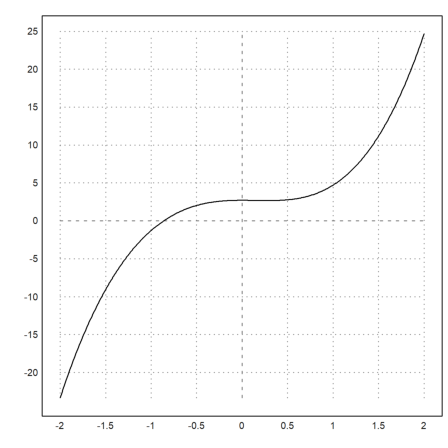
\includegraphics[keepaspectratio]{images/EMT4Kalkulus - Naila Khalidatus Salwa-008.png}}
\caption{images/EMT4Kalkulus\%20-\%20Naila\%20Khalidatus\%20Salwa-008.png}
\end{figure}

plot2d : fungsi ini digunakan untuk printah membuat plot dua dimensi

``f(x)'' : memanggil fungsi f(x)

-2,2 : grafik akan ditampilkan pada sb x dari rentang -2 sampai 2

Berikutnya kita definisikan fungsi:

\[g(x)=\frac{\sqrt{x^2-3x}}{x+1}\]\textgreater function g(x) := sqrt(x\^{}2-3*x)/(x+1)

\textgreater g(5)

\begin{verbatim}
0.527046276695
\end{verbatim}

\textgreater g(20)

\begin{verbatim}
0.878051853076
\end{verbatim}

\textgreater g(21)

\begin{verbatim}
0.883737367965
\end{verbatim}

\textgreater g(20:25)

\begin{verbatim}
[0.878052,  0.883737,  0.888915,  0.89365,  0.897998,  0.902003]
\end{verbatim}

Silakan Anda plot grafik fungsi di atas!

\textgreater aspect(1.5); plot2d(``g(x)'',20,25):

\begin{figure}
\centering
\pandocbounded{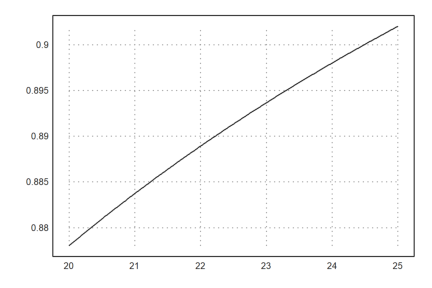
\includegraphics[keepaspectratio]{images/EMT4Kalkulus - Naila Khalidatus Salwa-010.png}}
\caption{images/EMT4Kalkulus\%20-\%20Naila\%20Khalidatus\%20Salwa-010.png}
\end{figure}

\textgreater f(g(5)) // komposisi fungsi

\begin{verbatim}
2.81254111152
\end{verbatim}

f(g(5)) adalah notasi yang menunjukkan komposisi fungsi.

Ini berarti kita akan melakukan dua langkah perhitungan:

Hitung g(5): Pertama, kita mencari nilai dari fungsi g ketika x = 5.

Hasilnya akan kita sebut sebagai a.

Hitung f(a): Selanjutnya, kita masukkan nilai a yang kita dapatkan dari langkah 1 ke dalam fungsi f.

Hasil akhir dari perhitungan ini adalah nilai dari f(g(5)).

\textgreater g(f(5))

\begin{verbatim}
0.993366510057
\end{verbatim}

\textgreater function h(x) := f(g(x)) // definisi komposisi fungsi

\textgreater h(5) // sama dengan f(g(5))

\begin{verbatim}
2.81254111152
\end{verbatim}

Silakan Anda plot kurva fungsi komposisi fungsi f dan g:

\[h(x)=f(g(x))\]dan

\[u(x)=g(f(x))\]bersama-sama kurva fungsi f dan g dalam satu bidang koordinat.

\textgreater f(0:10) // nilai-nilai f(0), f(1), f(2), \ldots, f(10)

\begin{verbatim}
[2.71828,  4.71653,  24.6596,  81.3716,  192.52,  376.328,  650.612,
1031.13,  1536.86,  2187.4,  3000.43]
\end{verbatim}

\textgreater fmap(0:10) // sama dengan f(0:10), berlaku untuk semua fungsi

\begin{verbatim}
[2.71828,  4.71653,  24.6596,  81.3716,  192.52,  376.328,  650.612,
1031.13,  1536.86,  2187.4,  3000.43]
\end{verbatim}

\textgreater gmap(20:25)

\begin{verbatim}
[0.878052,  0.883737,  0.888915,  0.89365,  0.897998,  0.902003]
\end{verbatim}

Misalkan kita akan mendefinisikan fungsi

\[f(x) = \begin{cases} x^3 & x>0 \\ x^2 & x\le 0. \end{cases}\]Fungsi tersebut tidak dapat didefinisikan sebagai fungsi numerik secara ``inline'' menggunakan format :=, melainkan didefinisikan sebagai program. Perhatikan, kata ``map'' digunakan agar fungsi dapat menerima vektor sebagai input, dan hasilnya berupa vektor. Jika tanpa kata ``map'' fungsinya hanya dapat menerima input satu nilai.

\textgreater function map f(x)

\begin{verbatim}
  if x>0 then return x^3
  else return x^2
  endif;
endfunction
\end{verbatim}

\textgreater f(4)

\begin{verbatim}
64
\end{verbatim}

\textgreater f(-2)

\begin{verbatim}
4
\end{verbatim}

\textgreater f(-5:5)

\begin{verbatim}
[25,  16,  9,  4,  1,  0,  1,  8,  27,  64,  125]
\end{verbatim}

\textgreater aspect(1.5); plot2d(``f(x)'',-5,5):

\begin{figure}
\centering
\pandocbounded{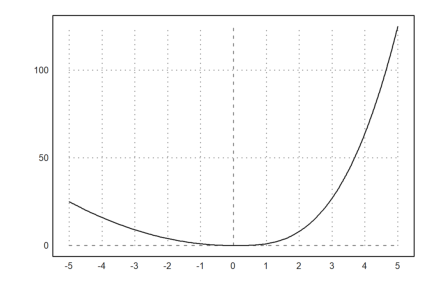
\includegraphics[keepaspectratio]{images/EMT4Kalkulus - Naila Khalidatus Salwa-014.png}}
\caption{images/EMT4Kalkulus\%20-\%20Naila\%20Khalidatus\%20Salwa-014.png}
\end{figure}

\[f(x)=2e^x\]\textgreater function f(x) \&= 2*E\^{}x; // fungsi simbolik

\textgreater\$f(a) // nilai fungsi secara simbolik

\[2\,e^{a}\]\textgreater function a:=12

\textgreater f(a)

\begin{verbatim}
325509.582838
\end{verbatim}

\textgreater{} f(E) // nilai fungsi berupa bilangan desimal

\begin{verbatim}
30.308524483
\end{verbatim}

\[g(x)=3x+1\]\textgreater function g(x) \&= 3*x+1

\begin{verbatim}
                               3 x + 1
\end{verbatim}

\textgreater g(50)

\begin{verbatim}
151
\end{verbatim}

\textgreater function h(x) \&= f(g(x)) // komposisi fungsi

\begin{verbatim}
                                 3 x + 1
                              2 E
\end{verbatim}

\textgreater{} plot2d(``h(x)'',-1,1):

\begin{figure}
\centering
\pandocbounded{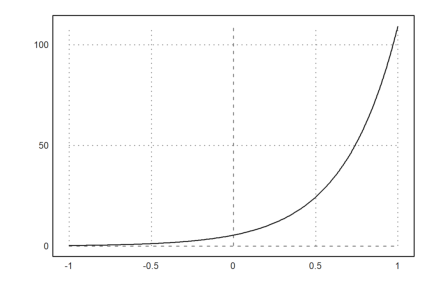
\includegraphics[keepaspectratio]{images/EMT4Kalkulus - Naila Khalidatus Salwa-018.png}}
\caption{images/EMT4Kalkulus\%20-\%20Naila\%20Khalidatus\%20Salwa-018.png}
\end{figure}

\section{Contoh Fungsi Aljabar}\label{contoh-fungsi-aljabar}

1.Diberikan fungsi:

\[f(x) = 6x^3+12\sqrt x\]Tentukan nilai f(1) dan f(4) kemudian cari nilai f(4)-2f(1)

Gambarkan juga grafiknya di f(1:4)!

\textgreater function f(x) := 6*x\^{}3+12*sqrt(x)

\textgreater f(1)

\begin{verbatim}
18
\end{verbatim}

\textgreater f(4)

\begin{verbatim}
408
\end{verbatim}

\textgreater f(4)-2*f(1)

\begin{verbatim}
372
\end{verbatim}

\textgreater aspect(1.5); plot2d(``f'',1,4):

\begin{figure}
\centering
\pandocbounded{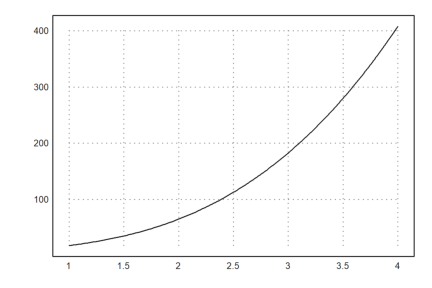
\includegraphics[keepaspectratio]{images/EMT4Kalkulus - Naila Khalidatus Salwa-020.png}}
\caption{images/EMT4Kalkulus\%20-\%20Naila\%20Khalidatus\%20Salwa-020.png}
\end{figure}

\begin{enumerate}
\def\labelenumi{\arabic{enumi}.}
\setcounter{enumi}{1}
\tightlist
\item
  Diberikan fungsi:
\end{enumerate}

\[k(x,y)= 12x^3+4y^2-3x+2\]Tentukan nilai k(1,1)+k(2,3)!

\textgreater function k(x,y):= 12*x\textsuperscript{3+4*y}2-3*x+2

\textgreater k(1,1)

\begin{verbatim}
15
\end{verbatim}

\textgreater k(2,3)

\begin{verbatim}
128
\end{verbatim}

\textgreater k(1,1)+k(2,3)

\begin{verbatim}
143
\end{verbatim}

\begin{enumerate}
\def\labelenumi{\arabic{enumi}.}
\setcounter{enumi}{2}
\tightlist
\item
  Diketahui suatu fungsi f(x,y,z) diddefinisikan sebagai betrikut
\end{enumerate}

\[f(x,y,z)=(3x-1)+\sqrt{x^3-y^2-z+6}\]Tentukan nilai f(3,4,5)!

\textgreater function f(x,y,z):= (3*x-1)+ sqrt(x\textsuperscript{3-y}2-z+6)

\textgreater f(3,4,5)

\begin{verbatim}
11.4641016151
\end{verbatim}

\section{Contoh Fungsi Trigonometri}\label{contoh-fungsi-trigonometri}

\begin{enumerate}
\def\labelenumi{\arabic{enumi}.}
\tightlist
\item
  Suatu fungsi trigonometri didefinisikan sebagai:
\end{enumerate}

\[f(x)=\frac{tan(x)}{2x+3x^2}\]Tentukan nilai dari f(6)-f(7)!

\textgreater function f(x):= tan(x)/2*x+3*x\^{}2

\textgreater f(6)-f(7)

\begin{verbatim}
-42.9230865137
\end{verbatim}

\begin{enumerate}
\def\labelenumi{\arabic{enumi}.}
\setcounter{enumi}{1}
\tightlist
\item
  Diberikan fungsi:
\end{enumerate}

\[f(x,y)=\frac{x^2+sin(y)}{xy}\]

Tentukan nilai f(4)!

\textgreater function f(x,y) := x\^{}2+sin(x)/x*y

\textgreater f(4,2)

\begin{verbatim}
15.6215987523
\end{verbatim}

\textgreater plot3d(``f'',-4,4):

\begin{figure}
\centering
\pandocbounded{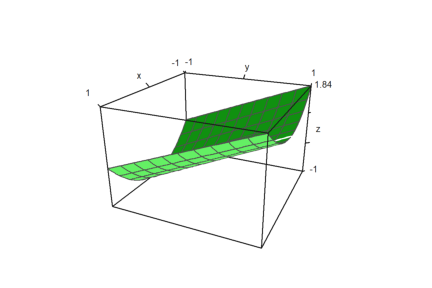
\includegraphics[keepaspectratio]{images/EMT4Kalkulus - Naila Khalidatus Salwa-025.png}}
\caption{images/EMT4Kalkulus\%20-\%20Naila\%20Khalidatus\%20Salwa-025.png}
\end{figure}

\begin{enumerate}
\def\labelenumi{\arabic{enumi}.}
\setcounter{enumi}{2}
\tightlist
\item
  Diberikan suatu fungsi
\end{enumerate}

\[f(x,y,z)=\frac{sin(x)}{cos(z)+sin(x)}+tan(y)\]tentukan nilai f(x,y,z) bila x=1, y=2, dan z=-3!

\textgreater function f(x,y,z)\&= sin(x)/(sin(x)+cos(z))+tan(y); \$f(x,y,z)

\[\frac{\sin x}{\cos z+\sin x}+\tan y\]\textgreater f(1,2,-3)

\begin{verbatim}
-7.85069041214
\end{verbatim}

\section{Contoh Fungsi Eksponensial}\label{contoh-fungsi-eksponensial}

\begin{enumerate}
\def\labelenumi{\arabic{enumi}.}
\tightlist
\item
  Diberikan sebuah fungsi f(x) sebagai berikut:
\end{enumerate}

\[f(x)=3^x\]Tentukan nilai f(x+1)-f(x)!

\textgreater function f(x)\&= 3\^{}x;

\textgreater\$f(x+1)

\[3^{x+1}\]\textgreater\$f(x)

\[3^{x}\]\textgreater\$f(x+1)-f(x)

\[2\,3^{x}\]2. Fungsi f(m) didefinisikan sebagai:

\[f(m)=27+8^m\]Tentukan nilai dari f(3), 2f(5), dan f(3)/2f(5)

\textgreater function f(m)\&=27+8\^{}m;

\textgreater\$f(3)

\[539\]\textgreater\$2*f(5)

\[65590\]\textgreater\$f(3)/(2*f(5))

\[\frac{77}{9370}\]3. Diketahui nilai y dari fungsi di bawah ini adalah 1

\[f(x)=2^{4x-12y}\]Tentukan nilai f(3), f(8), dan buat grafiknya di f(3:5)!

\textgreater function f(x):=2\^{}(4*x-12*y)

\textgreater function y:=1

\textgreater f(8)

\begin{verbatim}
1048576
\end{verbatim}

\textgreater f(3)

\begin{verbatim}
1
\end{verbatim}

\textgreater f(3:5)

\begin{verbatim}
[1,  16,  256]
\end{verbatim}

\textgreater aspect(1.3); plot2d(``f'',3,5):

\begin{figure}
\centering
\pandocbounded{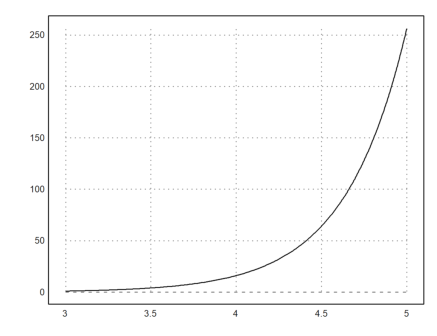
\includegraphics[keepaspectratio]{images/EMT4Kalkulus - Naila Khalidatus Salwa-037.png}}
\caption{images/EMT4Kalkulus\%20-\%20Naila\%20Khalidatus\%20Salwa-037.png}
\end{figure}

\section{Contoh Fungsi Logaritma}\label{contoh-fungsi-logaritma}

\begin{enumerate}
\def\labelenumi{\arabic{enumi}.}
\tightlist
\item
  Diberikan fungsi di bawah ini:
\end{enumerate}

\[f(x)=e^2 \cdot \left( \frac{1}{3+4 \log(x)}+\frac{1}{7} \right)\]Tentukan nilai f(0.6)!

\textgreater function f(x):= E\^{}2*(1/(3+4*log(x))+1/7)

\textgreater f(0.6)

\begin{verbatim}
8.77908249441
\end{verbatim}

\textgreater plot2d(``f'',-0.6,0.6):

\begin{figure}
\centering
\pandocbounded{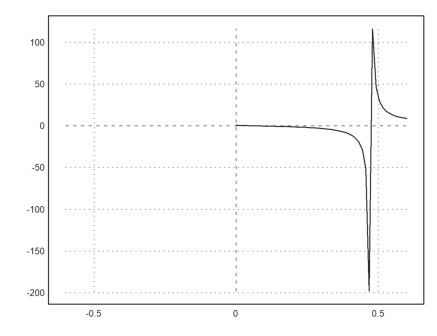
\includegraphics[keepaspectratio]{images/EMT4Kalkulus - Naila Khalidatus Salwa-039.png}}
\caption{images/EMT4Kalkulus\%20-\%20Naila\%20Khalidatus\%20Salwa-039.png}
\end{figure}

\section{Contoh Komposisi Fungsi}\label{contoh-komposisi-fungsi}

\begin{enumerate}
\def\labelenumi{\arabic{enumi}.}
\tightlist
\item
  Untuk fungsi:
\end{enumerate}

\[f(x) = x^2-3x+2\]\[g(x)=3x+5\]cari nilai

\[fog(-2), gof(0)\]\textgreater function f(x) := x\^{}2-3*x+2; \$f(x)

\textgreater function g(x) := 3*x+5; \$g(x)

\textgreater f(g(-2)), g(f(0))

\begin{verbatim}
6
11
\end{verbatim}

\textgreater{} plot2d(``(3*x+5)\^{}2-3*(3*x+5)+2'',-2,2):

\begin{figure}
\centering
\pandocbounded{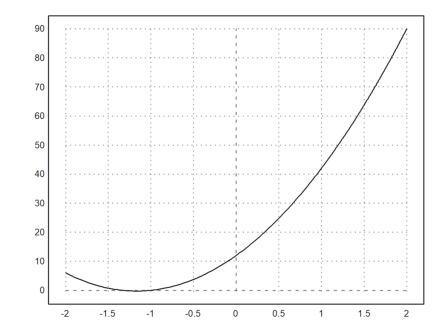
\includegraphics[keepaspectratio]{images/EMT4Kalkulus - Naila Khalidatus Salwa-043.png}}
\caption{images/EMT4Kalkulus\%20-\%20Naila\%20Khalidatus\%20Salwa-043.png}
\end{figure}

\chapter{Latihan}\label{latihan}

\begin{enumerate}
\def\labelenumi{\arabic{enumi}.}
\tightlist
\item
  Diberikan fungsi:
\end{enumerate}

\[b(x)= \frac{12x^3}{7x^2-3x}\]Cari nilai b(1), vektor b(1:4), dan buatkan grafiknya!

\textgreater function b(x) := 12*x\textsuperscript{3/(7*x}2-3*x); \$b(x)

\textgreater b(1)

\begin{verbatim}
3
\end{verbatim}

\textgreater b(1:4)

\begin{verbatim}
[3,  4.36364,  6,  7.68]
\end{verbatim}

\textgreater plot2d(``b'',-2,2):

\begin{figure}
\centering
\pandocbounded{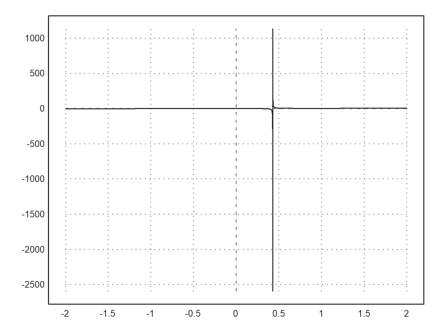
\includegraphics[keepaspectratio]{images/EMT4Kalkulus - Naila Khalidatus Salwa-045.png}}
\caption{images/EMT4Kalkulus\%20-\%20Naila\%20Khalidatus\%20Salwa-045.png}
\end{figure}

\begin{enumerate}
\def\labelenumi{\arabic{enumi}.}
\setcounter{enumi}{1}
\tightlist
\item
  Diketahui suatu fungsi f(x) sebagai berikut:
\end{enumerate}

\[f(x,y)=\frac{3(x-1)(y-2)}{2}+\frac{(y-2)(x-3)}{2}-2(x-1)(y-3)\]Tentukan nilai dari f(20,10) dan buat grafiknya di f(20,10:30,20)!

\textgreater function f(x,y) := 3*(x-1)*(y-2)/2+(y-2)*(x-3)/2 - 2*(x-1)*(y-3); \$f(x,y)

\textgreater f(20,10)

\begin{verbatim}
30
\end{verbatim}

\textgreater plot3d(``f'', 20,30,10,20):

\begin{figure}
\centering
\pandocbounded{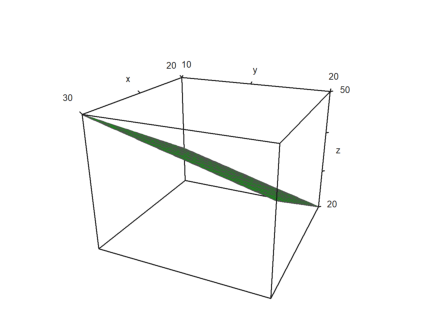
\includegraphics[keepaspectratio]{images/EMT4Kalkulus - Naila Khalidatus Salwa-047.png}}
\caption{images/EMT4Kalkulus\%20-\%20Naila\%20Khalidatus\%20Salwa-047.png}
\end{figure}

\begin{enumerate}
\def\labelenumi{\arabic{enumi}.}
\setcounter{enumi}{2}
\tightlist
\item
  Sketsakan grafik fungsi dibawah ini pada{[}-pi,2pi{]}
\end{enumerate}

\[y(t)=sin(5t)\]\textgreater function y(t) := sin(5*t)

\textgreater plot2d(``y'',-pi,pi):

\begin{figure}
\centering
\pandocbounded{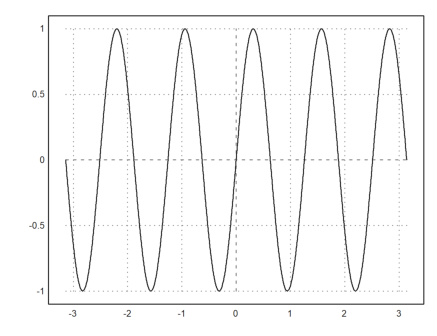
\includegraphics[keepaspectratio]{images/EMT4Kalkulus - Naila Khalidatus Salwa-049.png}}
\caption{images/EMT4Kalkulus\%20-\%20Naila\%20Khalidatus\%20Salwa-049.png}
\end{figure}

\begin{enumerate}
\def\labelenumi{\arabic{enumi}.}
\setcounter{enumi}{3}
\tightlist
\item
  Diketahui suatu fungsi f(x):
\end{enumerate}

\[f(x)=3^x\]Tentukan nilai f(a+2\^{}b-c) jika nilai a=1, b=2, dan c=5!

\textgreater function f(x) := 3\^{}x

\textgreater a:=1; b:= 2; c :=5; f(a+2\^{}b-c)

\begin{verbatim}
1
\end{verbatim}

\begin{enumerate}
\def\labelenumi{\arabic{enumi}.}
\setcounter{enumi}{4}
\tightlist
\item
  Untuk fungsi:
\end{enumerate}

\[f(x) = 2x^2-3x+20\]\[g(x)= 3x-5\]cari nilai

\[fog(5), gof(8)\]\textgreater function f(x):= 2*x\^{}2-3*x+20

\textgreater function g(x):= 3*x-5

\textgreater f(g(5))

\begin{verbatim}
190
\end{verbatim}

\textgreater g(f(8))

\begin{verbatim}
367
\end{verbatim}

\chapter{2. Limit}\label{limit}

\section{Definisi limit}\label{definisi-limit}

Pada dasarnya, limit digunakan untuk menyatakan sesuatu yang nilainya mendekati nilai tertentu. Limit dapat diartikan sebagai menuju suatu batas, sesuatu yang dekat namun tidak dapat dicapai. Mengapa nilainya hanya mendekati? Karena suatu fungsi biasanya tidak terdefinisi pada titik-titik tertentu. Walaupun suatu fungsi seringkali tidak terdefinisi untuk titik tertentu, namun masih dapat dicari tahu berapa nilai yang didekati oleh fungsi tersebut apabila titik tertentu semakin didekati yaitu dengan limit.

Bentuk umum dari limit sendiri dinotasikan dengan:

\[\lim_{x\rightarrow c}{F\left(x\right)}=L\]Notasi tersebut menyatakan bahwa f(x) untuk niai x mendekati c sama dengan L. F(x) disini dapat berupa bermacam-macam jenis fungsi. Dan L dapat berupa konstanta, ataupun ``und'' (tak terdefinisi), ``ind'' (tak tentu namun terbatas), ``infinity'' (kompleks tak hingga). Begitupun dengan batas c, dapat berupa sebarang nilai atau pada tak hingga (-inf, minf, dan inf).

Sebuah fungsi dapat dikatakan memiliki limit apabila limit kanan dan limit kiri nya memiliki nilai yang sama. Dimana, limit dari fungsi tersebut adalah nilai dari limit kanan dan limit kiri fungsi yang bernilai sama tadi.

\section{Sifat-sifat Limit}\label{sifat-sifat-limit}

Jika f(x) dan g(x) adalah fungsi yang memiliki limit di c, n merupakan bilangan bulat positif, dan k adalah konstanta.

\begin{enumerate}
\def\labelenumi{\arabic{enumi}.}
\tightlist
\item
\end{enumerate}

\[\lim_{x \to c}k=k\]\textgreater\$showev('limit(5,x,2))

\[5=5\]\[\lim_{x \to 2}5=5\]2.

maxima: 'limit(x,x,c)=c

\[\lim_{x\rightarrow c}{x}=c\]\textgreater\$showev('limit(x,x,3))

\[\lim_{x\rightarrow 3}{x}=3\]3.

maxima: 'limit(kf(x),x,c)= k*maxima: 'limit(f(x),x,c)

\[\lim_{x\rightarrow c}{{\it kf}\left(x\right)}=k\,\left(\lim_{x  \rightarrow c}{8^{x}+27}\right)\]\textgreater\$showev('limit(4*x\^{}2,x,1))

\[4\,\left(\lim_{x\rightarrow 1}{x^2}\right)=4\]4.

maxima: 'limit({[}g(x)+f(x){]},x,c)= maxima: 'limit(g(x),x,c) + maxima: 'limit(f(x),x,c)

\[\lim_{x\rightarrow c}{\left[ 8^{x}+3\,x+28 \right] }=\lim_{x  \rightarrow c}{8^{x}+27}+\lim_{x\rightarrow c}{3\,x+1}\]\textgreater\$showev('limit(x\^{}3+2*x,x,1))

\[\lim_{x\rightarrow 1}{x^3+2\,x}=3\]5.

maxima: 'limit({[}g(x)-f(x){]},x,c)= maxima: 'limit(g(x),x,c) - maxima: 'limit(f(x),x,c)

\[\lim_{x\rightarrow c}{\left[ -8^{x}+3\,x-26 \right] }=\lim_{x  \rightarrow c}{3\,x+1}-\lim_{x\rightarrow c}{8^{x}+27}\]\textgreater\$showev('limit(x\^{}2-4*x,x,5))

\[\lim_{x\rightarrow 5}{x^2-4\,x}=5\]6.

maxima: 'limit({[}g(x)*f(x){]},x,c)= maxima: 'limit(g(x),x,c) * maxima: 'limit(f(x),x,c)

\[\lim_{x\rightarrow c}{\left[ \left(3\,x+1\right)\,\left(8^{x}+27  \right) \right] }=\left(\lim_{x\rightarrow c}{3\,x+1}\right)\,\left(  \lim_{x\rightarrow c}{8^{x}+27}\right)\]\textgreater\$showev('limit((x-1)*(x+4),x,3))

\[\lim_{x\rightarrow 3}{\left(x-1\right)\,\left(x+4\right)}=14\]7.

maxima: 'limit(g(x)/f(x),x,c)= maxima: 'limit(g(x),x,c) / maxima: 'limit(f(x),x,c)

\[\lim_{x\rightarrow c}{\frac{3\,x+1}{8^{x}+27}}=\frac{\lim_{x  \rightarrow c}{3\,x+1}}{\lim_{x\rightarrow c}{8^{x}+27}}\]\textgreater\$showev('limit((x+5)/(x+1),x,0))

\[\lim_{x\rightarrow 0}{\frac{x+5}{x+1}}=5\]8.

maxima: 'limit(f(x)\textsuperscript{n,x,c)=maxima:'limit(f(x),x,c)}n

\[\lim_{x\rightarrow c}{\left(8^{x}+27\right)^{n}}=\left(\lim_{x  \rightarrow c}{8^{x}+27}\right)^{n}\]\textgreater\$showev('limit((x+3)\^{}2,x,1))

\[\lim_{x\rightarrow 1}{\left(x+3\right)^2}=16\]9.

\[\lim_{x\rightarrow c}{\left(8^{x}+27\right)^{\frac{1}{n}}}=\left(  \lim_{x\rightarrow c}{8^{x}+27}\right)^{\frac{1}{n}}\]\textgreater\$showev('limit((x\textsuperscript{2+3*x+1)}(1/2),x,2))

\[\lim_{x\rightarrow 2}{\sqrt{x^2+3\,x+1}}=\sqrt{11}\]\#\# Limit pada EMT

Pada EMT cara mendefinisikan limit yaitu dengan format :

\$showev('limit(f(x),x,c))

Format tersebut akan menampilkan limit yang dimaksud dan hasilnya. Jika kita ingin menampilkan hasilnya saja dari sebuah limit tanpa menampilkan limitnya, kita bisa menggunakan format :

\$limit(f(x),x,c)

Sedangkan, untuk limit kanan dan limit kiri seperti pada definisi dapat ditampilkan di EMT dengan cara menambah opsi ``plus'' atau ``minus'' :

\$showev('limit(f(x),x,c, plus)) atau 'limit(f(x),x,c, minus)

\textgreater\$showev('limit(x\^{}2+3*x+4,x,2))

\[\lim_{x\rightarrow 2}{x^2+3\,x+4}=14\]\textgreater\$limit(x\^{}2+3*x+4,x,2)

\[14\]\#\# Menghitung dan Visualisasi Limit

Perhitungan limit pada EMT dapat dilakukan dengan menggunakan fungsi Maxima, yakni ``limit''. Fungsi ``limit'' dapat digunakan untuk menghitung limit fungsi dalam bentuk ekspresi maupun fungsi yang sudah didefinisikan sebelumnya. Nilai limit dapat dihitung pada sebarang nilai atau pada tak hingga (-inf, minf, dan inf). Limit kiri dan limit kanan juga dapat dihitung, dengan cara memberi opsi ``plus'' atau ``minus''. Hasil limit dapat berupa nilai, ``und'' (tak definisi), ``ind'' (tak tentu namun terbatas), ``infinity'' (kompleks tak hingga).

Limit dapat divisualisasikan menggunakan plot 2 dimensi. Pada EMT sendiri, format yang bisa digunakan untuk memvisualisasikan limit adalah :

plot2d(``f(x)'',-c,c):

Dengan f(x) adalah fungsi pada limit yang dicari, dan c berupa bilangan real menyesuaikan batas dari limit itu sendiri.

\section{Limit Aljabar}\label{limit-aljabar}

\begin{enumerate}
\def\labelenumi{\arabic{enumi}.}
\tightlist
\item
  Tunjukkan bahwa limit kiri dan kanan dari fungsi berikut bernilai sama. Berapakah nilai limitnya?
\end{enumerate}

\[\lim_{x\rightarrow 0}{x^2+x-1}\]\textgreater\$showev('limit(x\^{}2+x-1,x,0,minus))

\[\lim_{x\uparrow 0}{x^2+x-1}=-1\]\textgreater\$showev('limit(x\^{}2+x-1,x,0,plus))

\[\lim_{x\downarrow 0}{x^2+x-1}=-1\]Dapat terlihat bahwa nilai limit kiri = nilai limit kanan. Maka fungsi tersebut memiliki nilai limit, yaitu :

\textgreater\$showev('limit(x\^{}2+x-1,x,0))

\[\lim_{x\rightarrow 0}{x^2+x-1}=-1\]2. Tunjukkan bahwa limit kiri dan kanan dari fungsi berikut bernilai sama. Berapakah nilai limitnya?

\[\lim_{x\rightarrow 3}{\sqrt{x^2+x-1}}\]\textgreater\$showev('limit(sqrt(x\^{}2+x-1),x,3,minus))

\[\lim_{x\uparrow 3}{\sqrt{x^2+x-1}}=\sqrt{11}\]\textgreater\$showev('limit(sqrt(x\^{}2+x-1),x,3,plus))

\[\lim_{x\downarrow 3}{\sqrt{x^2+x-1}}=\sqrt{11}\]Dapat terlihat bahwa nilai limit kiri = nilai limit kanan. Maka fungsi tersebut memiliki nilai limit, yaitu :

\textgreater\$showev('limit(sqrt(x\^{}2+x-1),x,3))

\[\lim_{x\rightarrow 3}{\sqrt{x^2+x-1}}=\sqrt{11}\]3. Tunjukkan bahwa limit kiri dan kanan dari fungsi berikut bernilai sama. Berapakah nilai limitnya?

\[\lim_{x\rightarrow -3}{\frac{\left| x+3\right| }{x+3}}\]\textgreater\$showev('limit(abs(x+3)/(x+3),x,-3,minus))

\[\lim_{x\uparrow -3}{\frac{\left| x+3\right| }{x+3}}=-1\]\textgreater\$showev('limit(abs(x+3)/(x+3),x,-3,plus))

\[\lim_{x\downarrow -3}{\frac{\left| x+3\right| }{x+3}}=1\]Karena nilai limit kiri tidak sama dengan nilai limit kanan. Maka fungsi diatas tidak memiliki limit di x=-3

\textgreater\$showev('limit(abs(x+3)/(x+3),x,-3))

\[\lim_{x\rightarrow -3}{\frac{\left| x+3\right| }{x+3}}={\it und}\]\textgreater\$limit(x\^{}3+4*x+5,x,2)

\[21\]\textgreater plot2d(``x\^{}3+4*x+5'',1.8,2.2); plot2d(2,21,\textgreater points,style=``ow'',\textgreater add):

\begin{figure}
\centering
\pandocbounded{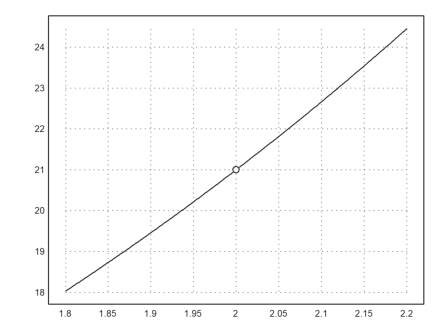
\includegraphics[keepaspectratio]{images/EMT4Kalkulus - Naila Khalidatus Salwa-089.png}}
\caption{images/EMT4Kalkulus\%20-\%20Naila\%20Khalidatus\%20Salwa-089.png}
\end{figure}

Jadi berdasarkan grafik, nilai limit tersebut adalah 21.

\begin{enumerate}
\def\labelenumi{\arabic{enumi}.}
\setcounter{enumi}{4}
\tightlist
\item
  Berapakah nilai limit dari fungsi berikut? Tunjukkan dengan menggunakan grafik!
\end{enumerate}

maxima: 'limit((abs(x-5))/(x-5),x,5)

\[\lim_{x\rightarrow 5}{\frac{\left| x-5\right| }{x-5}}\]\textgreater plot2d(``abs(x-5)/(x-5)'',4.9,5.1):

\begin{figure}
\centering
\pandocbounded{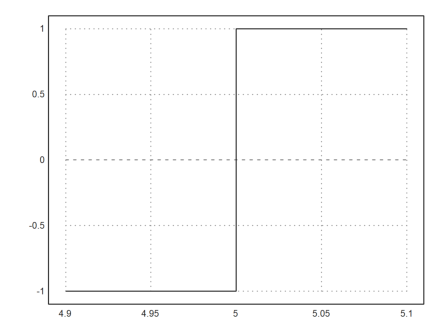
\includegraphics[keepaspectratio]{images/EMT4Kalkulus - Naila Khalidatus Salwa-091.png}}
\caption{images/EMT4Kalkulus\%20-\%20Naila\%20Khalidatus\%20Salwa-091.png}
\end{figure}

Karena nilai limit kiri tidak sama dengan limit kanan. maka nili limit fungsi tersebut tidak ada.

\begin{enumerate}
\def\labelenumi{\arabic{enumi}.}
\setcounter{enumi}{5}
\tightlist
\item
  Berapakah nilai limit dari fungsi berikut?
\end{enumerate}

\[\lim_{x\rightarrow \infty }{\frac{x^5-3\,x^3+x^2-9}{4\,x^5-7\,x^4+2  \,x-1}}\]\textgreater\$showev('limit((x\textsuperscript{5-3*x}3+x\textsuperscript{2-9)/(4*x}5-7*x\^{}4+2*x-1),x,inf))

\[\lim_{x\rightarrow \infty }{\frac{x^5-3\,x^3+x^2-9}{4\,x^5-7\,x^4+2  \,x-1}}=\frac{1}{4}\]7. Tunjukkan nilai limit fungsi berikut dengan grafik!

maxima: 'limit(sqrt(x\^{}2+x)-x,x,inf)

\[\lim_{x\rightarrow \infty }{\sqrt{x^2+x}-x}\]\textgreater plot2d(``sqrt(x\^{}2+x)-x'',0,10):

\begin{figure}
\centering
\pandocbounded{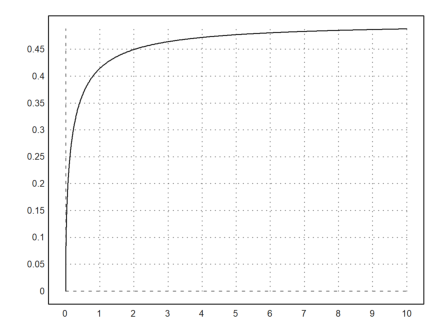
\includegraphics[keepaspectratio]{images/EMT4Kalkulus - Naila Khalidatus Salwa-095.png}}
\caption{images/EMT4Kalkulus\%20-\%20Naila\%20Khalidatus\%20Salwa-095.png}
\end{figure}

Dengan menggunakan grafik diperlihatkan bahwa nilai limit mendekati 0.5. Mari kita buktikan di baris perintah

\textgreater\$showev('limit(sqrt(x\^{}2+x)-x,x,inf))

\[\lim_{x\rightarrow \infty }{\sqrt{x^2+x}-x}=\frac{1}{2}\]\#\# Limit Trigonometri

\begin{enumerate}
\def\labelenumi{\arabic{enumi}.}
\tightlist
\item
  Tunjukkan bahwa limit kiri dan kanan dari fungsi berikut bernilai sama. Berapakah nilai limitnya?
\end{enumerate}

\[\lim_{x\rightarrow 0}{\cos x\,\sin x}\]\textgreater\$showev('limit(cos(x)*sin(x),x,0,minus))

\[\lim_{x\uparrow 0}{\cos x\,\sin x}=0\]\textgreater\$showev('limit(cos(x)*sin(x),x,0,plus))

\[\lim_{x\downarrow 0}{\cos x\,\sin x}=0\]Dapat terlihat bahwa nilai limit kiri = nilai limit kanan. Maka fungsi tersebut memiliki nilai limit, yaitu :

\textgreater\$showev('limit(cos(x)*sin(x),x,0))

\[\lim_{x\rightarrow 0}{\cos x\,\sin x}=0\]2. Berapakah nilai limit dari fungsi berikut? Tunjukkan dengan menggunakan grafik

\[\lim_{x\rightarrow 0}{\frac{1-\cos x}{x}}\]\textgreater plot2d(``(1-cos(x))/x'',-pi/4,pi/4); plot2d(0,0,\textgreater points,style=``ow'',\textgreater add):

\begin{figure}
\centering
\pandocbounded{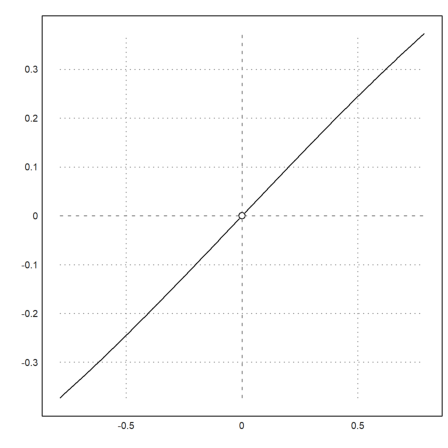
\includegraphics[keepaspectratio]{images/EMT4Kalkulus - Naila Khalidatus Salwa-102.png}}
\caption{images/EMT4Kalkulus\%20-\%20Naila\%20Khalidatus\%20Salwa-102.png}
\end{figure}

\begin{enumerate}
\def\labelenumi{\arabic{enumi}.}
\setcounter{enumi}{2}
\tightlist
\item
  Tunjukkan bahwa limit kiri dan kanan dari fungsi berikut bernilai sama. Berapakah nilai limitnya?
\end{enumerate}

\[\lim_{x\rightarrow 0}{\frac{\sin x}{1-\cos x}}\]\textgreater\$showev('limit(3*sin(x)\^{}2/(1-cos(x)),x,0,minus))

\[3\,\left(\lim_{x\uparrow 0}{\frac{\sin ^2x}{1-\cos x}}\right)=6\]\textgreater\$showev('limit(3*sin(x)\^{}2/(1-cos(x)),x,0,plus))

\[3\,\left(\lim_{x\downarrow 0}{\frac{\sin ^2x}{1-\cos x}}\right)=6\]Dapat terlihat bahwa nilai limit kiri = nilai limit kanan. Maka fungsi tersebut memiliki nilai limit, yaitu

\textgreater\$showev('limit(3*sin(x)\^{}2/(1-cos(x)),x,0))

\[3\,\left(\lim_{x\rightarrow 0}{\frac{\sin ^2x}{1-\cos x}}\right)=6\]4. Berapakah nilai limit dari fungsi berikut? Tunjukkan dengan menggunakan grafik!

\[\lim_{x\rightarrow 0}{\left| \sin \left(2\,x\right)\right| -\cos x}\]\textgreater\$limit(abs(sin(2*x))-cos(x),x,0)

\[-1\]\textgreater plot2d(``abs(sin(2x))-cos(x)'',-pi/2,pi/2); plot2d(0,-1,\textgreater points,style=``ow'',\textgreater add):

\begin{figure}
\centering
\pandocbounded{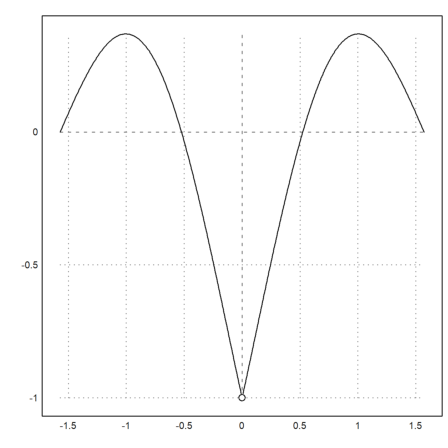
\includegraphics[keepaspectratio]{images/EMT4Kalkulus - Naila Khalidatus Salwa-109.png}}
\caption{images/EMT4Kalkulus\%20-\%20Naila\%20Khalidatus\%20Salwa-109.png}
\end{figure}

Jadi berdasarkan grafik, nilai limit tersebut adalah -1.

\begin{enumerate}
\def\labelenumi{\arabic{enumi}.}
\setcounter{enumi}{4}
\tightlist
\item
  Berapakah nilai limit dari fungsi berikut? Tunjukkan dengan menggunakan grafik!
\end{enumerate}

maxima: 'limit(2\emph{sin(x)}cos(x)-tan(x),x,pi/3)

\[\lim_{x\rightarrow \frac{\pi}{3}}{2\,\cos x\,\sin x-\tan x}\]\textgreater\$limit(2*cos(x)*sin(x)-tan(x),x,pi/3)

\[-\frac{\sqrt{3}}{2}\]\textgreater plot2d(``2*cos(x)*sin(x)-tan(x)'',0,pi/2.9); plot2d(pi/3,-(3)\^{}(1/2)/2,\textgreater points,style=``ow'',\textgreater add):

\begin{figure}
\centering
\pandocbounded{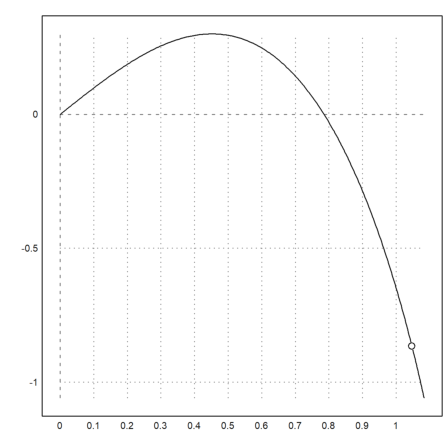
\includegraphics[keepaspectratio]{images/EMT4Kalkulus - Naila Khalidatus Salwa-112.png}}
\caption{images/EMT4Kalkulus\%20-\%20Naila\%20Khalidatus\%20Salwa-112.png}
\end{figure}

Jadi berdasarkan grafik, nilai limit tersebut adalah -0.866.

\begin{enumerate}
\def\labelenumi{\arabic{enumi}.}
\setcounter{enumi}{5}
\tightlist
\item
  Berapakah nilai limit dari fungsi berikut? Tunjukkan dengan menggunakan grafik!
\end{enumerate}

\[2\,\left(\lim_{x\rightarrow 0}{\sec x}\right)\]\textgreater\$limit(2*sec(x),x,0)

\[2\]\textgreater plot2d(``2*sec(x)'',-pi/3,pi/3); plot2d(0,2,\textgreater points,style=``ow'',\textgreater add):

\begin{figure}
\centering
\pandocbounded{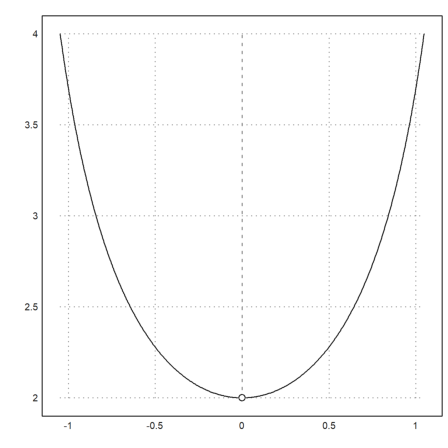
\includegraphics[keepaspectratio]{images/EMT4Kalkulus - Naila Khalidatus Salwa-115.png}}
\caption{images/EMT4Kalkulus\%20-\%20Naila\%20Khalidatus\%20Salwa-115.png}
\end{figure}

Jadi berdasarkan grafik, nilai limit tersebut adalah 2.

\section{Latihan}\label{latihan-1}

Tunjukkan bahwa limit kiri dan kanan dari fungsi berikut bernilai sama!

\[\lim_{x\rightarrow 3}{\frac{\left(x-3\right)\,\left| x^3+5\,x+8  \right| }{\cos x}}\]\textgreater\$limit(abs(x\^{}3+5*x+8)/cos(x)*(x-3),x,3)

\[0\]Tunjukkan nilai limit fungsi berikut dengan menggunakan grafik!

\[\lim_{x\rightarrow 0.8}{\frac{\left(x^2+6\,x+1\right)\,\sin \left(3  \,x\right)}{\cos x}}\]\textgreater\$limit((x\^{}2+6*x+1)*sin(3*x)/cos(x),x,0.8)

\[6.243635699770241\]\# 3. Turunan Fungsi

Turunan adalah pengukuran terhadap bagaimana fungsi berubah seiring

perubahan nilai yang dimasukkan, atau secara umum turunan menunjukkan bagaimana suatu besaran berubah akibat perubahan besaran lainnya. Proses dalam menemukan turunan disebut diferensiasi.

Definisi turunan:

\[f'(x) = \lim_{h\to 0}\frac{f(x+h)-f(x)}{h}\]

Berikut adalah contoh-contoh menentukan turunan fungsi dengan beberapa cara.

\section{Turunan fungsi Aljabar}\label{turunan-fungsi-aljabar}

Mencari turunan dari

\[f(x)=x^n\]\textgreater\$showev('limit(((x+h)\textsuperscript{n-x}n)/h,h,0)) // turunan x\^{}n

\[\lim_{h\rightarrow 0}{\frac{\left(x+h\right)^{n}-x^{n}}{h}}=n\,x^{n  -1}\]Bukti:

\[(x+h)^n= \binom{n}{0}x^{n-0}h^0+ \binom{n}{1}x^{n-1}h^1+\binom{n}{2}x^{n-2}h^2+...+\binom{n}{n}x^{n-n}h^n\]\[(x+h)^n = x^n+nx^{n-1}h+\binom{n}{2}x^{n-2}h^2+...+h^n\]\[(x+h)^n -x^n = nx^{n-1}h+\binom{n}{2}x^{n-2}h^2+...+h^n\]\[\frac{(x+h)^n -x^n}{h} = nx^{n-1}+\binom{n}{2}x^{n-2}h+...+h^{n-1}\]\[ \lim_{h\to 0}\frac{(x+h)^n -x^n}{h}=nx^{n-1}\]Mencari turunan dari

\[f(x)=x^2\]\textgreater\$showev('limit(((x+h)\textsuperscript{2-x}2)/h,h,0)) // turunan x\^{}2

\[\lim_{h\rightarrow 0}{\frac{\left(x+h\right)^2-x^2}{h}}=2\,x\]\textgreater p \&= expand((x+h)\textsuperscript{2-x}2)\textbar simplify; \$p //pembilang dijabarkan dan disederhanakan

\[2\,h\,x+h^2\]\textgreater q \&=ratsimp(p/h); \$q // ekspresi yang akan dihitung limitnya disederhanakan

\[2\,x+h\]\textgreater\$limit(q,h,0) // nilai limit sebagai turunan

\[2\,x\]\textgreater plot2d({[}``x\^{}2'', ``2x''{]}, color={[}black,red{]}):

\begin{figure}
\centering
\pandocbounded{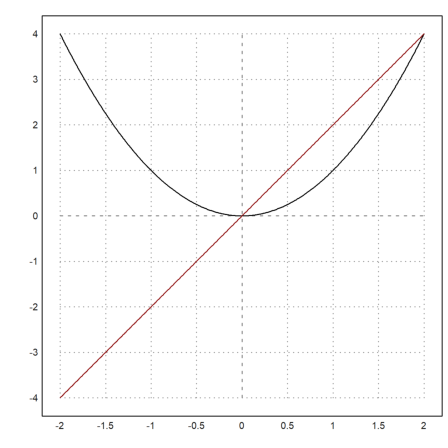
\includegraphics[keepaspectratio]{images/EMT4Kalkulus - Naila Khalidatus Salwa-133.png}}
\caption{images/EMT4Kalkulus\%20-\%20Naila\%20Khalidatus\%20Salwa-133.png}
\end{figure}

Mencari turunan dari

\[f(x)=x^x\]\textgreater function f(x) \&= x\^{}x

\begin{verbatim}
                                   x
                                  x
\end{verbatim}

\textgreater\$showev('limit(f(x+h)-f(x)/h,h,0))

\[\lim_{h\rightarrow 0}{\left(x+h\right)^{x+h}-\frac{x^{x}}{h}}=  {\it infinity}\]Di sini Maxima bermasalah terkait limit:

\[\lim_{h\to 0} \frac{(x+h)^{x+h}-x^x}{h}.\]Dalam hal ini diperlukan asumsi nilai x.

\textgreater\&assume(x\textgreater0); \$showev('limit((f(x+h)-f(x))/h,h,0)) // turunan f(x)=f(x)\^{}x

\[\lim_{h\rightarrow 0}{\frac{\left(x+h\right)^{x+h}-x^{x}}{h}}=x^{x}  \,\left(\log x+1\right)\]\textgreater\&forget(x\textgreater0) // jangan lupa, lupakan asumsi untuk kembali ke semula

\begin{verbatim}
                               [x &gt; 0]
\end{verbatim}

\textgreater\&forget(x\textless0)

\begin{verbatim}
                               [x &lt; 0]
\end{verbatim}

\textgreater\&facts()

\begin{verbatim}
                                  []
\end{verbatim}

Mencari turunan dari

\[f(x)=\frac{1}{x}\]\textgreater\$showev('limit((1/(x+h)-1/x)/h,h,0)) // turunan 1/x

\[\lim_{h\rightarrow 0}{\frac{\frac{1}{x+h}-\frac{1}{x}}{h}}=-\frac{1  }{x^2}\]\textgreater plot2d(``-x\^{}(-2)'', color=red):

\begin{figure}
\centering
\pandocbounded{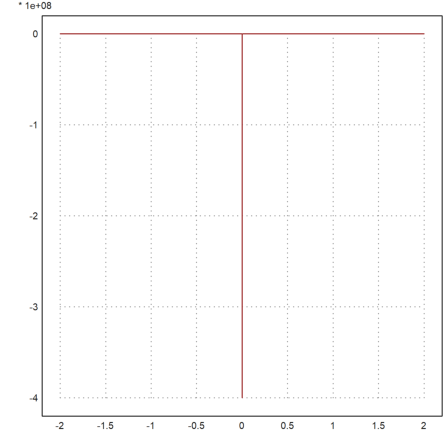
\includegraphics[keepaspectratio]{images/EMT4Kalkulus - Naila Khalidatus Salwa-140.png}}
\caption{images/EMT4Kalkulus\%20-\%20Naila\%20Khalidatus\%20Salwa-140.png}
\end{figure}

\textgreater{}

\section{Turunan fungsi trigonometri}\label{turunan-fungsi-trigonometri}

Mencari turunan dari

\[sin(x)\]\textgreater\$showev('limit((sin(x+h)-sin(x))/h,h,0)) // turunan sin(x)

\[\lim_{h\rightarrow 0}{\frac{\sin \left(x+h\right)-\sin x}{h}}=\cos   x\]Bukti:

\[sin(x+h) = sin(x)cos(h)+cos(x)sin(h)\]\[sin(x+h)-sin(x) = sin(x)cos(h)+cos(x)sin(h)-sin(x)\]\[sin(x+h)-sin(x) = cos(x)sin(h) - sin(x)+sin(x)cos(h)\]\[sin(x+h)-sin(x) = cos(x)sin(h) - sin(x)(1-cos(h))\]\[\lim_{h\to 0}\frac{sin(x+h)-sin(x)}{h}= \lim_{h\to 0}\frac{cos(x)sin(h)}{h}-\lim_{h\to 0}\frac{sin(x)(1-cos(h)}{h}\]\[\lim_{h\to 0}\frac{sin(x+h)-sin(x)}{h}=cos(x)\lim_{h\to 0}\frac{sin(h)}{h}-sin(x)\lim_{h\to 0}\frac{(1-cos(h)}{h}\]\[=cos(x)\times 1 -sin(x) \times 0 =cos(x)\]\textgreater p \&= expand((sin(x+h)-sin(x)))\textbar simplify; \$p

\[\sin \left(x+h\right)-\sin x\]\textgreater q \&=ratsimp(p/h); \$q

\[\frac{\sin \left(x+h\right)-\sin x}{h}\]\textgreater\$limit(q,h,0) // nilai limit sebagai turunan

\[\cos x\]\textgreater plot2d({[}``sin(x)'', ``cos(x)''{]},0, 2*pi, color={[}blue,green{]}):

\begin{figure}
\centering
\pandocbounded{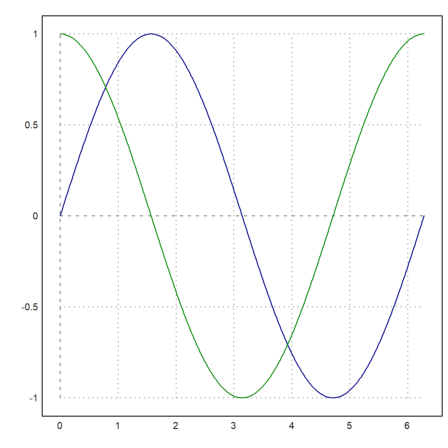
\includegraphics[keepaspectratio]{images/EMT4Kalkulus - Naila Khalidatus Salwa-153.png}}
\caption{images/EMT4Kalkulus\%20-\%20Naila\%20Khalidatus\%20Salwa-153.png}
\end{figure}

Mencari turunan dari

\[tan(x)\]\textgreater\$showev('limit((tan(x+h)-tan(x))/h,h,0)) // turunan tan(x)

\[\lim_{h\rightarrow 0}{\frac{\tan \left(x+h\right)-\tan x}{h}}=  \frac{1}{\cos ^2x}\]Bukti:

\[tan(x+h) = \frac {tan (x)+tan (h)}{1-tan(x)tan(h)}\]\[tan(x+h)-tan (x) ={\frac {tan (x)+tan (h)-tan (x)+tan^2(x)tan(h)}{1-tan(x)tan(h)}}\]\[\frac {tan(x+h)-tan (x)}{h} =\frac{ \frac {tan (x)+tan (h)-tan (x)+tan^2(x)tan(h)}{1-tan(x)tan(h)}}{h}\]\[= \frac {tan(h)+tan^2(x) tan(h)}{h(1-tan(x)tan(h)}\]\[= \lim_{h\to 0} \frac {tan(h)+tan^2(x) tan(h)}{h(1-tan(x)tan(h)}\]\[= \lim_{h\to 0} \frac {1 +tan^2(x)}{1-tan (x)tan(h)} \cdot \lim_{h\to 0} \frac{tan (h)}{h}\]\[= \frac {1 +tan^2(x)}{1-tan (x)tan(0)} \cdot 1\]\[= 1+tan^2(x)\]\[1+tan^2(x)=1+ \frac{sin^2(x)}{cos^2(x)}\]\[= \frac{cos^2(x) + sin^2(x)}{cos^2(x)}\]\[= \frac{1}{cos^2(x)}\]\textgreater p \&= expand((tan(x+h)-tan(x)))\textbar simplify; \$p

\[\tan \left(x+h\right)-\tan x\]\textgreater q \&=ratsimp(p/h); \$q

\[\frac{\tan \left(x+h\right)-\tan x}{h}\]\textgreater\$limit(q,h,0) // nilai limit sebagai turunan

\[\frac{1}{\cos ^2x}\]Mencari turunan dari

\[arcsin(x)\]\[f'(x) = \lim_{A-B \to 0} \frac {A-B}{2 sin [\frac{A-B}{2}] cos [\frac{A+B}{2}]}\]\[f'(x) = \lim_{A-B \to 0} \frac {\frac{2(A-B)}{2}}{2 sin [\frac{A-B}{2}] cos [\frac{A+B}{2}]}\]ingat bahwa

\[\lim_{x \to 0} \frac{x}{sin (x)}=1\]\[f'(x) = \lim_{A-B \to 0}\frac{\frac{(A-B)}{2}}{sin [\frac{A-B}{2}]} \cdot \frac{2}{2cos [\frac{A+B}{2}]}\]\[f'(x) = 1 \cdot \frac{2}{2cos [\frac{B+B}{2}]}\]\[f'(x) = \frac {1}{cos (B)}\]\[f'(x) = \frac {1}{\sqrt{(cos^2 (B)}}\]\[f'(x) = \frac {1}{\sqrt{(1- sin^2 (B)}}= \frac {1}{\sqrt{(1-x^2}}\]\textgreater\$showev('limit((asin(x+h)-asin(x))/h,h,0)) // turunan arcsin(x)

\[\lim_{h\rightarrow 0}{\frac{\arcsin \left(x+h\right)-\arcsin x}{h}}=  \frac{1}{\sqrt{1-x^2}}\]Bukti:

\[f'(x)= \lim_{h\to 0} \frac {arcsin(x+h)-arcsin(x)}{h}\]Misalkan arcsin(x+h)=A dan arcsin(x)=B

Sehingga sin A= x+h dan sin B=x

Kurangkan persamaan kedua dengan persamaan pertama

\[sin(A)-sin(B)=(x+h)-x\]\[sin(A)-sin(B) = h\]karena

\[h \to 0, sin(A)-sin(B) \to 0\]

maka

\[sin(A)\to sin(B),  A \to B, A-B \to 0\]sehingga f'(x) menjadi

\[f'(x) = \lim_{A-B \to 0} \frac{A-B}{sin A- sin B}\]Identitas trigonometri

\[sin(A)-sin(B) = 2 sin[\frac{A-B}{2}]cos[\frac{A+B}{2}]\]\textgreater p \&= expand((asin(x+h)-asin(x)))\textbar simplify; \$p //pembilang dijabarkan dan disederhanakan

\[\arcsin \left(x+h\right)-\arcsin x\]\textgreater q \&=ratsimp(p/h); \$q // ekspresi yang akan dihitung limitnya disederhanakan

\[\frac{\arcsin \left(x+h\right)-\arcsin x}{h}\]\textgreater\$limit(q,h,0) // nilai limit sebagai turunan

\[\frac{1}{\sqrt{1-x^2}}\]\textgreater plot2d({[}``asin(x)'',``1/(sqrt(1-x\^{}2))''{]},0,2*pi,color={[}blue,red{]}):

\begin{figure}
\centering
\pandocbounded{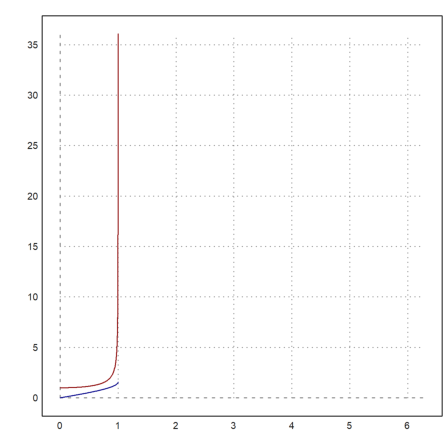
\includegraphics[keepaspectratio]{images/EMT4Kalkulus - Naila Khalidatus Salwa-190.png}}
\caption{images/EMT4Kalkulus\%20-\%20Naila\%20Khalidatus\%20Salwa-190.png}
\end{figure}

Mencari turunan dari

\[x^2+10\]

di titik x=5

\textgreater function f(x) \&= x\^{}2+10 // definisikan f(x)=x\^{}2+10

\begin{verbatim}
                                2
                               x  + 10
\end{verbatim}

\textgreater function df(x) \&= showev('diff(f(x),x)); \$df(x)

\[\frac{d}{d\,x}\,\left(x^2+10\right)=2\,x\]\textgreater\$\% with x=5

\[{\it \%at}\left(\frac{d}{d\,x}\,\left(x^2+10\right) , x=5\right)=10\]\textgreater diff(f,5), diffc(f,5)

\begin{verbatim}
9.99999999997
10
\end{verbatim}

Mencari turunan dari

\[sinh(x)\]\textgreater function f(x) \&= sinh(x) // definisikan f(x)=sinh(x)

\begin{verbatim}
                               sinh(x)
\end{verbatim}

\textgreater function df(x) \&= limit((f(x+h)-f(x))/h,h,0); \$df(x) // df(x) = f'(x)

\[\frac{e^ {- x }\,\left(e^{2\,x}+1\right)}{2}\]Hasilnya adalah cosh(x), karena

\[\frac{e^x+e^{-x}}{2}=\cosh(x).\]\textgreater plot2d({[}``f(x)'',``df(x)''{]},-pi,pi,color={[}blue,red{]}):

\begin{figure}
\centering
\pandocbounded{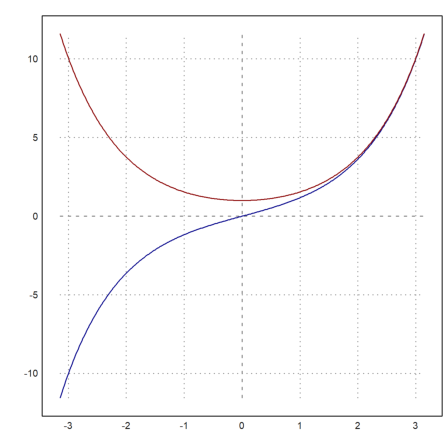
\includegraphics[keepaspectratio]{images/EMT4Kalkulus - Naila Khalidatus Salwa-197.png}}
\caption{images/EMT4Kalkulus\%20-\%20Naila\%20Khalidatus\%20Salwa-197.png}
\end{figure}

\textgreater\$showev('diff(f(x),x))

\[\frac{d}{d\,x}\,\sinh x=\cosh x\]\textgreater\$\% with x=3

\[{\it \%at}\left(\frac{d}{d\,x}\,\sinh x , x=3\right)=\cosh 3\]\textgreater\$float(\%)

\[{\it \%at}\left(\frac{d^{1.0}}{d\,x^{1.0}}\,\sinh x , x=3.0\right)=  10.06766199577777\]\textgreater plot2d(f,0,3.1):

\begin{figure}
\centering
\pandocbounded{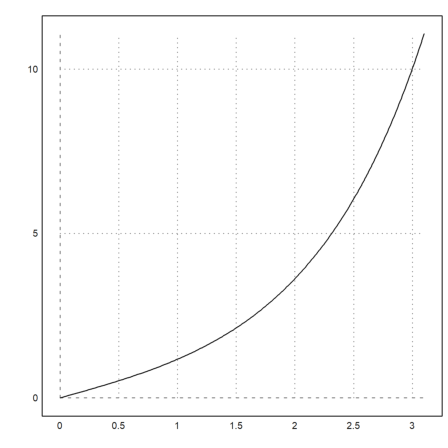
\includegraphics[keepaspectratio]{images/EMT4Kalkulus - Naila Khalidatus Salwa-201.png}}
\caption{images/EMT4Kalkulus\%20-\%20Naila\%20Khalidatus\%20Salwa-201.png}
\end{figure}

Mencari turunan dari

\[f(x)=sin(3x^5+7)^2\]\textgreater function f(x) \&= sin(3*x\textsuperscript{5+7)}2

\begin{verbatim}
                               2    5
                            sin (3 x  + 7)
\end{verbatim}

\textgreater\$showev('diff(f(x),x))

\[\frac{d}{d\,x}\,\sin ^2\left(3\,x^5+7\right)=30\,x^4\,\cos \left(3  \,x^5+7\right)\,\sin \left(3\,x^5+7\right)\]Kita akan mencari nilai turunan tersebut ketika x=2

\textgreater\$\% with x = 2

\[{\it \%at}\left(\frac{d}{d\,x}\,\sin ^2\left(3\,x^5+7\right) , x=2  \right)=480\,\cos 103\,\sin 103\]\textgreater\$float(\%)

\[{\it \%at}\left(\frac{d^{1.0}}{d\,x^{1.0}}\,\sin ^2\left(3.0\,x^5+  7.0\right) , x=2.0\right)=-233.9140567500984\]\textgreater diff(f,2), diffc(f,2)

\textgreater plot2d(f,0,3.1) :

\begin{figure}
\centering
\pandocbounded{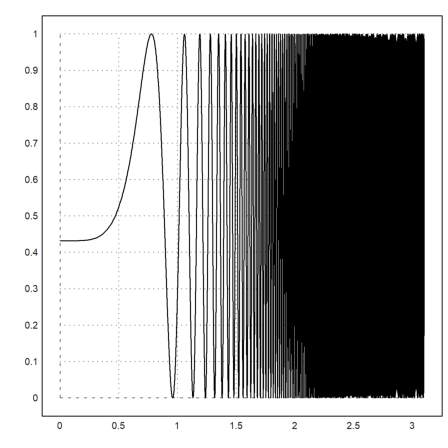
\includegraphics[keepaspectratio]{images/EMT4Kalkulus - Naila Khalidatus Salwa-206.png}}
\caption{images/EMT4Kalkulus\%20-\%20Naila\%20Khalidatus\%20Salwa-206.png}
\end{figure}

Mencari turunan dari

\[a(x)=5cos(2x)-2xsin(2x)\]\textgreater function a(x) \&=5*cos(2*x)-2*x*sin(2*x) // mendifinisikan fungsi a

\begin{verbatim}
                      5 cos(2 x) - 2 x sin(2 x)
\end{verbatim}

\textgreater function da(x) \&=diff(a(x),x); \$da(x) // da(x) = a'(x)

\[-12\,\sin \left(2\,x\right)-4\,x\,\cos \left(2\,x\right)\]\textgreater\$'a(1)=a(1), \$float(a(1)), \$'a(2)=a(2), \$float(a(2)) // nilai a(1) dan a(2)

\[-0.2410081230863468\]\pandocbounded{
\includegraphics[keepaspectratio]{images/EMT4Kalkulus - Naila Khalidatus Salwa-210.png}}

\textgreater xp=solve(``da'',1,2,0) // solusi a'(x)=0 pada interval {[}1, 2{]}

\begin{verbatim}
1.35822987384
\end{verbatim}

\textgreater da(xp), a(xp) // cek bahwa a'(xp)=0 dan nilai ekstrim di titik tersebut

\begin{verbatim}
0
-5.67530133759
\end{verbatim}

\textgreater plot2d({[}``a(x)'',``da(x)''{]},0,2*pi,color={[}blue,red{]}): //grafik fungsi dan turunannya

\begin{figure}
\centering
\pandocbounded{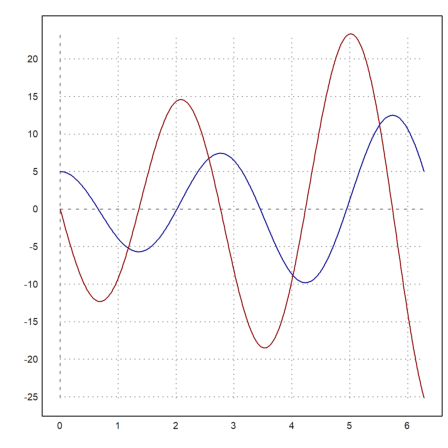
\includegraphics[keepaspectratio]{images/EMT4Kalkulus - Naila Khalidatus Salwa-211.png}}
\caption{images/EMT4Kalkulus\%20-\%20Naila\%20Khalidatus\%20Salwa-211.png}
\end{figure}

Pada titik puncak grafik a(x), nilai turunan a'(x) akan selalu sama dengan nol. Ini karena gradien garis singgung pada titik puncak adalah nol.

\section{Turunan fungsi logaritma}\label{turunan-fungsi-logaritma}

Mencari turunan dari

\[f(x)= log(x)\]\textgreater\$showev('limit((log(x+h)- log(x))/h,h,0)) // turunan log(x)

\[\lim_{h\rightarrow 0}{\frac{\log \left(x+h\right)-\log x}{h}}=  \frac{1}{x}\]Bukti:

\[f'(x) = \lim_{h\to 0} \frac{log(x+h)-log x}{h}\]ingat bahwa

\[log(a)-log(b)= log (\frac{a}{b})\]\[f'(x)=\lim_{h\to 0}\frac{ log (\frac{x+h}{x})}{h}\]\[f'(x)=\lim_{h\to 0}\frac{ log (1 + \frac{h}{x})}{h}\]misalkan h/x = n sehingga h=nx

\[f'(x)=\lim_{n\to 0}\frac{ log (1 + n)}{nx}\]\[f'(x)=\lim_{n\to 0}\frac{1}{nx} \cdot log(1+n)\]ingat bahwa

\[a log b = log b^a\]\[f'(x)=\lim_{n\to 0} \frac{1}{x} \cdot log(1+n)^\frac{1}{n}\]\[f'(x)= \frac{1}{x}log \lim_{n\to 0}(1+n)^\frac{1}{n}\]\[\lim_{n\to 0}(1+n)^\frac{1}{n} = e\]\[f'(x)= \frac{1}{x}log e\]\[f'(x)=\frac{1}{x}\]\textgreater\$showev('limit((log((x+h)/(x)))/h,h,0))//definisi logaritma

\[\lim_{h\rightarrow 0}{\frac{\log \left(\frac{x+h}{x}\right)}{h}}=  \frac{1}{x}\]\textgreater\$showev('limit(((h/x))/h,h,0))//menggunakan identitas logaritma, sisanya adalah hasil turunan

\[\frac{1}{x}=\frac{1}{x}\]\textgreater plot2d({[}``log(x)'', ``1/x''{]},-1,1, color={[}red,lightgreen{]}):

\begin{figure}
\centering
\pandocbounded{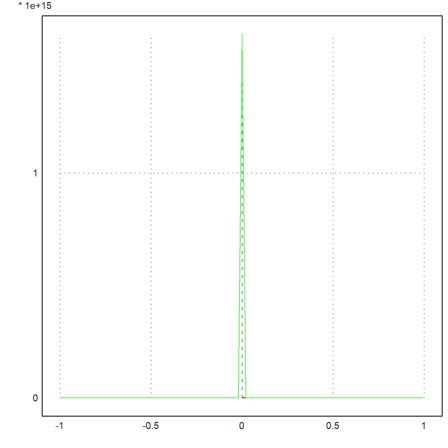
\includegraphics[keepaspectratio]{images/EMT4Kalkulus - Naila Khalidatus Salwa-228.png}}
\caption{images/EMT4Kalkulus\%20-\%20Naila\%20Khalidatus\%20Salwa-228.png}
\end{figure}

\section{Turunan fungsi eksponensial}\label{turunan-fungsi-eksponensial}

Mencari turunan dari

\[f(x)=e^x\]\textgreater\$showev('limit((E\textsuperscript{(x+h)-E}x)/h,h,0)) // turunan f(x)=e\^{}x

\begin{verbatim}
Answering "Is x an integer?" with "integer"
Answering "Is x an integer?" with "integer"
Answering "Is x an integer?" with "integer"
Answering "Is x an integer?" with "integer"
Answering "Is x an integer?" with "integer"
Maxima is asking
Acceptable answers are: yes, y, Y, no, n, N, unknown, uk
Is x an integer?

Use assume!
Error in:
 $showev('limit((E^(x+h)-E^x)/h,h,0)) // turunan f(x)=e^x ...
                                     ^
\end{verbatim}

Maxima bermasalah dengan limit:

\[\lim_{h\to 0}\frac{e^{x+h}-e^x}{h}.\]Oleh karena itu diperlukan trik khusus agar hasilnya benar.

\textgreater\$showev('factor(E\textsuperscript{(x+h)-E}x))

\[{\it factor}\left(e^{x+h}-e^{x}\right)=\left(e^{h}-1\right)\,e^{x}\]\textgreater\$showev('limit(factor((E\textsuperscript{(x+h)-E}x)/h),h,0)) // turunan f(x)=e\^{}x

\[\left(\lim_{h\rightarrow 0}{\frac{e^{h}-1}{h}}\right)\,e^{x}=e^{x}\]\textgreater\$showev('limit((E\^{}h-1)/h,h,0))

\[\lim_{h\rightarrow 0}{\frac{e^{h}-1}{h}}=1\]\#\# Sifat- sifat Turunan

\begin{enumerate}
\def\labelenumi{\arabic{enumi}.}
\item
  Jika f(x)=k dengan k suatu konstanta maka untuk sebarang x, f'x = 0

  Bukti:
\end{enumerate}

\[f'(x)= \lim_{h\to 0}\frac{f(x+h)-f(x)}{h} = \lim_{h\to 0}\frac{k-k}{h} = \lim_{h\to 0}0=0\]2. Jika f(x)=x, maka f'(x)=1

Bukti:

\[f'(x)= \lim_{h\to 0}\frac{f(x+h)-f(x)}{h} = \lim_{h\to 0}\frac{x+h-x}{h}=\lim_{h\to 0}\frac {h}{h}=1\]3. Jika k suatu konstanta dan f suatu fungsi yang terdiferensialkan,

maka (kf)`(x)= kf'(x)

Bukti:

Andaikan F(x) = kf(x), maka

\[F'(x)=\lim_{h\to 0}\frac{F(x+h)-F(x)}{h}=\lim_{h\to 0}\frac{kf(x+h)-kf(x)}{h}\]\[    = \lim_{h\to 0}k \frac{f(x+h)-f(x)}{h}=k\lim_{h\to 0}\frac{f(x+h)-f(x)}{h}\]\[= kf'(x)\]4. Jika f dan g adalah fungsi-fungsi yang terdiferensial,

maka (f+g)`(x)=f'(x)+g'(x)

Bukti:

\[F'(x)=\lim_{h\to 0}\frac{f(x+h)+g(x+h)-f(x)+g(x)}{h}\]\[=\lim_{h\to 0}[\frac{f(x+h)-f(x)}{h}+\frac{g(x+h)-g(x)}{h}]\]\[=\lim_{h\to 0}\frac{f(x+h)-f(x)}{h}+\lim_{h\to 0}\frac{g(x+h)-g(x)}{h}=f'(x)+g'(x)\]5. Andaikan f dan g adalah fungsi yang dapat didiferensialkan,

maka (fg)`(x)=f'(x)g(x)+ f(x)g'(x)

Bukti:

Andaikan F(x)=f(x)g(x)

\[F'(x)= \lim_{h\to 0}\frac{F(x+h)-F(x)}{h}\]\[= \lim_{h\to 0}\frac{f(x+h)g(x+h)-f(x)g(x)}{h}\]\[= \lim_{h\to 0}\frac{f(x+h)g(x+h)-f(x+h)g(x)+f(x+h)g(x)-f(x)g(x)}{h}\]\[=\lim_{h\to 0}[f(x+h)\frac{g(x+h)-g(x)+g(x)f(x+h)-f(x)}{h}]\]\[=\lim_{h\to 0} f(x+h)=\lim_{h \to 0}\frac{g(x+h)-g(x)}{h}+g(x)\lim_{h\to 0}\frac{f(x+h)-f(x)}{h}\]\[=f(x)g'(x)+g(x)f'(x)\]6. Andaikan f dan g adalah fungsi yang dapat didiferensialkan

dengan g(x)tidak sama dengan 0, maka:

\[(\frac{f}{g})(x)=\frac{g(x)f'(x)-f(x)g'(x)}{g(x)^2}\] Bukti:\\
Andaikan F(x)=f(x)/g(x)

\[F'(x)= \lim_{h\to 0}\frac{F(x+h)-F(x)}{h}\]\[= \lim_{h\to 0}\frac{\frac{f(x+h)}{g(x+h}-\frac{f(x)}{g(x)}}{h}\]\[= \lim_{h\to 0}\frac{g(x)f(x+h)-f(x)g(x+h)}{h}\frac{1}{g(x)g(x+h)}\]\[= \lim_{h\to 0}[\frac{g(x)f(x+h)-g(x)f(x)+g(x)f(x)-f(x)g(x+h)}{h}\frac{1}{g(x)g(x+h)}]\]\[=\lim_{h\to 0} [g(x)\frac{f(x+h)-f(x)}{h}-f(x)\frac{g(x+h)-g(x)}{h}]\frac{1}{g(x)g(x+h)}\]\[=[g(x)f'(x)-f(x)g'(x)]\frac{1}{g(x)g(x)}\]\[=\frac{g(x)f'(x)-f(x)g'(x)}{g(x)^2}\]\#\# Aplikasi turunan

\begin{enumerate}
\def\labelenumi{\arabic{enumi}.}
\tightlist
\item
  Persamaan gerak suatu partikel dinyatakan dengan rumus
\end{enumerate}

\[s=f(t)=(3t+1)^{\frac{1}{2}}\] ( s dalam meter dan t dalam detik).\\
Kecepatan partikel tersebut pada saat t=8 adalah \ldots{} m/detik.

Penyelesaian:

\textgreater function f(t) \&= (3*t+1)\^{}(1/2); \$f(t)

\[\sqrt{3\,t+1}\]\textgreater function df(t) \&= diff(f(t),t); \$df(t)

\[\frac{3}{2\,\sqrt{3\,t+1}}\]\textgreater\$df(8); fraction \%

\[\frac{3}{10}\] Jadi, kecepatan partikel tersebut pada saat t=8 adalah 3/10 m/detik.

\begin{enumerate}
\def\labelenumi{\arabic{enumi}.}
\setcounter{enumi}{1}
\tightlist
\item
  Sebuah pabrik baju memerlukan x meter kain untuk diproduksi yang dinyatakan dengan fungsi:
\end{enumerate}

\[P(x)={\frac{1}{3}}x^2-12x+150\] (dalam juta rupiah).\\
Berapa biaya produksi minimum yang dikeluarkan oleh pabrik baju

tersebut?

Penyelesaian:

\textgreater function P(x) \&= (1/3)*x\^{}2-12*x+150; \$P(x)

\[\frac{x^2}{3}-12\,x+150\]\textgreater function dP(x) \&= diff(P(x),x); \$dP(x)

\[\frac{2\,x}{3}-12\] P(x) akan bernilai minimum jika P'(x)=0, maka:

\textgreater\$dP(x)=0

\[\frac{2\,x}{3}-12=0\]\textgreater\$\&solve(dP(x),x)

\[\left[ x=18 \right] \] Dengan demikian, biaya produksinya adalah:

\textgreater P(18)

\begin{verbatim}
42
\end{verbatim}

Jadi, biaya produksi minimum yang dikeluarkan oleh pabrik tersebut

adalah 42 juta rupiah.

\begin{enumerate}
\def\labelenumi{\arabic{enumi}.}
\setcounter{enumi}{2}
\item
  Sebuah peluru ditembakkan ke atas. Jika tinggi h meter setelah t

  detik dirumuskan dengan
\end{enumerate}

\[h(t)=120t-5t^2\] maka berapa tinggi maksimum yang dicapai peluru tersebut?

Penyelesaian:\\
Diketahui:

\[h(t)=120t-5t^2\] Turunan pertama fungsi h adalah

\textgreater function h(t) \&= 120*t-5*t\^{}2; \$h(t)

\[120\,t-5\,t^2\]\textgreater function dh(t) \&= diff(h(t),t); \$dh(t)

\[120-10\,t\] Nilai t akan maksimum saat

\[h'(t)=0\]\textgreater\$dh(t)=0

\[120-10\,t=0\]\textgreater\$\&solve(dh(t),t)

\[\left[ t=12 \right] \] Ketinggian maksimum yang dapat dicapai peluru saat t=12, yaitu

\textgreater\$h(12)

\[720\] Jadi, ketinggian maksimum peluru adalah 720 meter.

\section{Soal-soal Latihan}\label{soal-soal-latihan}

\begin{enumerate}
\def\labelenumi{\arabic{enumi}.}
\tightlist
\item
  Cari f'(4) dari fungsi
\end{enumerate}

\[f(x) = \frac {2x-1}{x^2-x}\]\textgreater function f(x) \&= (2*x-1)/(x\^{}2-x); \$f(x)

\[\frac{2\,x-1}{x^2-x}\]\textgreater function df(x) \&= diff(f(x), x); \$df(x)

\[\frac{2}{x^2-x}-\frac{\left(2\,x-1\right)^2}{\left(x^2-x\right)^2}\]\textgreater df(4); fraction \%

\begin{verbatim}
-25/144
\end{verbatim}

\begin{enumerate}
\def\labelenumi{\arabic{enumi}.}
\setcounter{enumi}{1}
\tightlist
\item
  Cari turunan dari
\end{enumerate}

\[g(x)=x^2\cdot sin(x)\]\textgreater function g(x) \&= x\^{}2*sin(x); \$g(x)

\[x^2\,\sin x\]\textgreater function dg(x) \&= diff (g(x), x); \$dg(x)

\[2\,x\,\sin x+x^2\,\cos x\]3. Cari turunan dari

\[(4x-7)^2(2x+3)\]\textgreater function f(x) \&= (4*x-7)\^{}2*(2*x+3); \$f(x)

\[\left(2\,x+3\right)\,\left(4\,x-7\right)^2\]\textgreater function df(x) \&= diff(f(x), x); \$df(x)

\[2\,\left(4\,x-7\right)^2+8\,\left(2\,x+3\right)\,\left(4\,x-7  \right)\]\textgreater F \&= expand(df(x))\textbar simplify; \$F

\[96\,x^2-128\,x-70\]4. Temukan turunan dari

\[f(x)=ln(x^3+3x-4)\]\textgreater function f(x) \&= ln(x\^{}3+3*x-4); \$f(x)

\[\log \left(x^3+3\,x-4\right)\]\textgreater\$showev('diff(f(x),x))

\[\frac{d}{d\,x}\,\log \left(x^3+3\,x-4\right)=\frac{3\,x^2+3}{x^3+3  \,x-4}\]5. Tentukan turunan dari

\[f(x)=cos(5x)+sin(2x)\]\textgreater function f(x) \&= cos(5*x)+sin(2*x); \$f(x)

\[\cos \left(5\,x\right)+\sin \left(2\,x\right)\]\textgreater\$showev('diff(f(x),x))

\[\frac{d}{d\,x}\,\left(\cos \left(5\,x\right)+\sin \left(2\,x\right)  \right)=2\,\cos \left(2\,x\right)-5\,\sin \left(5\,x\right)\]6. Sebuah kembang api diluncurkan ke udara. Ketinggian kembang api

h=(t) (dalam meter) pada t sekon dimodelkan dengan

\[f(t)=16t^2+200t+4\] Tentukan kecepatan luncur kembang api saat t= 3 sekon.

Penyelesaian:

\textgreater function f(t) \&= 16*t\^{}2+200*t+4; \$f(t)

\[16\,t^2+200\,t+4\]\textgreater function df(t) \&= diff(f(t),t); \$df(t)

\[32\,t+200\]\textgreater\$df(3); fraction \%

\[296\]Jadi, kecepatan kembang api saat t=3 sekon adalah 296 m/s

\chapter{4. Integral Tak Tentu}\label{integral-tak-tentu}

EMT dapat digunakan untuk menghitung integral, baik integral tak tentu maupun integral tentu.

Pada notebook ini akan ditunjukkan perhitungan integral tentu dengan menggunakan Teorema Dasar Kalkulus:

Fungsi untuk menentukan integral adalah integrate. Fungsi ini dapat digunakan untuk menentukan, baik integral tentu maupun tak tentu (jika fungsinya memiliki antiderivatif).

\section{CAKUPAN PEMBAHASAN}\label{cakupan-pembahasan}

Definisi

Cara menulis integral pada EMT

Sifat-sifat

Rumus

Kurva

\section{DEFINISI}\label{definisi}

Integral Tak Tentu adalah bentuk integral yang variabel integrasinya tidak memiliki batas sehingga integrasi dari sebuah fungsi akan menghasilkan banyak kemungkinan dan hanya dinyatakan sebagai penyelesaian umum. Istilah tak tentu berarti bentuk fungsi F(x) memuat konstanta real sebarang.

Misalkan diketahui suatu fungsi F(x) yang merupakan fungsi umum yang memiliki sifat F'(x)=f(x), maka integral tak tentu merupakan himpunan anti turunan F(x) dari f(x) pada interval negatif tak hingga sampai positif tak hingga yang dinotasikan :

\[F(x) = \int f(x) dx+c\]\#\# MENULIS INTEGRAL PADA LATEX

Untuk menulis dengan Latex menggunakan fungsi \int

\[f(x)= \int x^3 dx\]\[\int 15x^7 dx\]\[\int x^4 dx\]\[\int 7x^3 dx\]\[\int 5x dx\]\#\# SIFAT INTEGRAL TAK TENTU

\begin{enumerate}
\def\labelenumi{\arabic{enumi}.}
\item
  Sifat Pangkat

  Jika n adalah sembarang bilangan rasional kecuali -1, maka integral tak tentu dari x\^{}n ditulis :
\end{enumerate}

\[\int x^n dx+c=\frac{x^{n+1}}{n+1} +c\]Contoh:

\[\int x^2 dx+c=\frac{x^{2+1}}{2+1} +c =\frac{x^3}{3} +c\]2. Penjumlahan dan Pengurangan

\[\int[g(x)+f(x)]dx = \int g(x) dx + \int f(x)dx\]\[\int [x^2+4x] dx = \int x^2 dx + \int 4x dx\]\[\int[g(x)-f(x)]dx = \int g(x) dx - \int f(x)dx\]\[\int [x^7-3x] dx = \int x^7 dx - \int 3x dx\]3. Perkalian

Bayangkan f(x) dan g(x) adalah dua fungsi yang bisa kita hitung integral tak tentu (artinya kita mencari antiturunannya), dan anggap k adalah suatu angka tetap (konstanta). Maka aturannya berlaku:

\[\int kf(x)dx=k \int f(x)dx\]\[\int 4x^2dx=4 \int x^2dx\]\#\# RUMUS INTEGRAL TAK TENTU

Integral tak tentu berarti nilai atau batasannya belum pasti, sehingga ada nilai konstanta(c) di dalamnya. Jadi rumus dasar integral tak tentu adalah :

\textgreater\$showev('integrate(x\^{}n,x)+c)

\begin{verbatim}
Answering "Is n equal to -1?" with "no"
\end{verbatim}

\[\int {x^{n}}{\;dx}+c=\frac{x^{n+1}}{n+1}+c\]\textgreater\$showev('integrate(x\^{}-1,x)+c)

\[\int {\frac{1}{x}}{\;dx}+c=\log x+c\]Integral dari fungsi

\[f(x)=x^{-1}\]

menghasilkan fungsi ln karena berasal dari teorema kalkulus

\section{KURVA FUNGSI INTEGRAL/ANTITURUNAN}\label{kurva-fungsi-integralantiturunan}

Kurva fungsi antiturunan adalah kurva yang menggambarkan hubungan antara suatu fungsi dan antiturunannya. Antiturunan, juga dikenal sebagai integral.

Jangan lupa untuk menuliskan terhadap variabel apa suatu fungsi tersebut diintegralkan

\begin{enumerate}
\def\labelenumi{\arabic{enumi}.}
\tightlist
\item
  kurva antiturunan dari fungsi aljabar
\end{enumerate}

\[ f(x)=4x^3 dx\]\textgreater\$showev('integrate(4*x\^{}3,x)+c)

\[4\,\int {x^3}{\;dx}+c=x^4+c\]\textgreater plot2d({[}``4*x\^{}3'', ``x\^{}4'', ``x\^{}4+1''{]}):

\begin{figure}
\centering
\pandocbounded{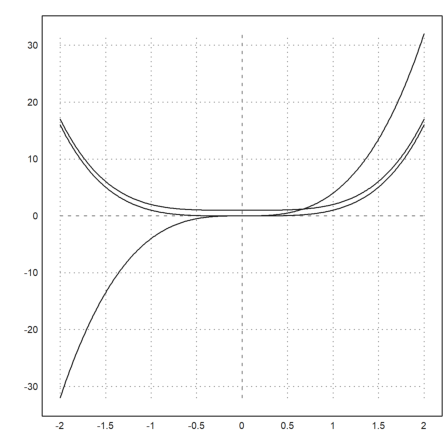
\includegraphics[keepaspectratio]{images/EMT4Kalkulus - Naila Khalidatus Salwa-312.png}}
\caption{images/EMT4Kalkulus\%20-\%20Naila\%20Khalidatus\%20Salwa-312.png}
\end{figure}

\begin{enumerate}
\def\labelenumi{\arabic{enumi}.}
\setcounter{enumi}{1}
\tightlist
\item
  kurva antiderivatif fungsi trigonometri dengan
\end{enumerate}

\[f(x)= cos(x)\]\textgreater\$showev('integrate(cos(x),x)+c)

\[\int {\cos x}{\;dx}+c=\sin x+c\]\textgreater plot2d({[}``cos(x)'', ``sin(x)'', ``sin(x)+1''{]}):

\begin{figure}
\centering
\pandocbounded{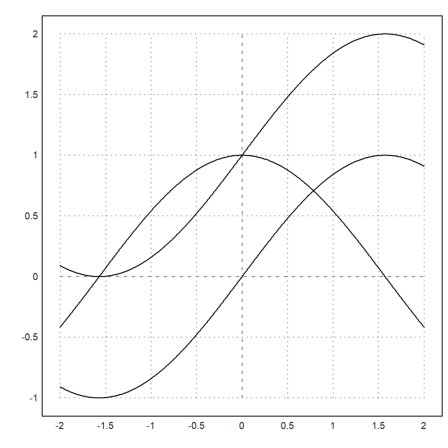
\includegraphics[keepaspectratio]{images/EMT4Kalkulus - Naila Khalidatus Salwa-315.png}}
\caption{images/EMT4Kalkulus\%20-\%20Naila\%20Khalidatus\%20Salwa-315.png}
\end{figure}

\begin{enumerate}
\def\labelenumi{\arabic{enumi}.}
\setcounter{enumi}{2}
\tightlist
\item
  kurva antiderivatif dari fungsi eksponensial dengan
\end{enumerate}

\[f(x)=x e^x\]\textgreater\$showev('integrate(x*E\^{}x,x)+c)

\[\int {x\,e^{x}}{\;dx}+c=\left(x-1\right)\,e^{x}+c\]\textgreater plot2d({[}``x*E\textsuperscript{x'',''(x-1)E}x+1'',``(x-1)E\textsuperscript{x+2'',''(x-1)E}x+3'',``(x-1)E\^{}x+4''{]}):

\begin{figure}
\centering
\pandocbounded{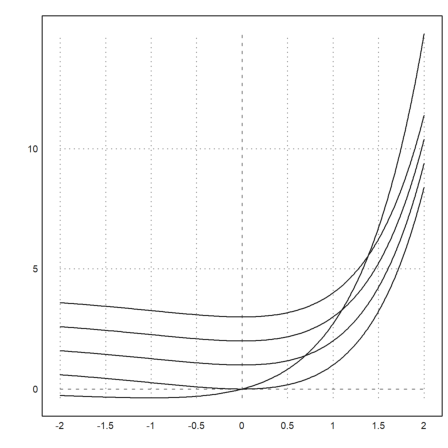
\includegraphics[keepaspectratio]{images/EMT4Kalkulus - Naila Khalidatus Salwa-318.png}}
\caption{images/EMT4Kalkulus\%20-\%20Naila\%20Khalidatus\%20Salwa-318.png}
\end{figure}

\begin{enumerate}
\def\labelenumi{\arabic{enumi}.}
\setcounter{enumi}{3}
\tightlist
\item
  kurva antiderivatif dari fungsi logaritma dengan
\end{enumerate}

\[f(x)=log(4x)\]\textgreater\$showev('integrate(log(4*x),x)+c)

\[\int {\log \left(4\,x\right)}{\;dx}+c=\frac{4\,x\,\log \left(4\,x  \right)-4\,x}{4}+c\]\textgreater plot2d({[}``log(4*x)'',``(4*x)log(4*x)-4*x/4 +1'',``(4*x)log(4*x)-4*x/4 +2'',``(4*x)log(4*x)-4*x/4 +3''{]}):

\begin{figure}
\centering
\pandocbounded{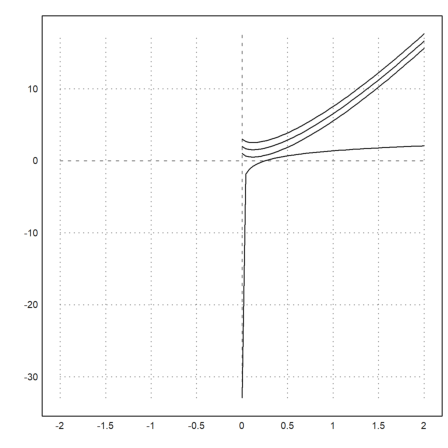
\includegraphics[keepaspectratio]{images/EMT4Kalkulus - Naila Khalidatus Salwa-321.png}}
\caption{images/EMT4Kalkulus\%20-\%20Naila\%20Khalidatus\%20Salwa-321.png}
\end{figure}

\section{LATIHAN SOAL}\label{latihan-soal}

\begin{enumerate}
\def\labelenumi{\arabic{enumi}.}
\tightlist
\item
  Tuliskan integral tak tentu dari fungsi aljabar berikut serta buatlah grafiknya :
\end{enumerate}

\[f(x)=x^5\]\textgreater\$showev('integrate(log(4*x),x)+c)

\[\int {\log \left(4\,x\right)}{\;dx}+c=\frac{4\,x\,\log \left(4\,x  \right)-4\,x}{4}+c\]\textgreater plot2d({[}``4*x\^{}3'', ``x\^{}4'', ``x\^{}4+1''{]}):

\begin{figure}
\centering
\pandocbounded{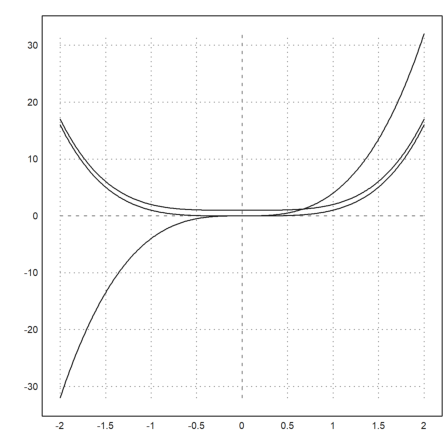
\includegraphics[keepaspectratio]{images/EMT4Kalkulus - Naila Khalidatus Salwa-324.png}}
\caption{images/EMT4Kalkulus\%20-\%20Naila\%20Khalidatus\%20Salwa-324.png}
\end{figure}

\begin{enumerate}
\def\labelenumi{\arabic{enumi}.}
\setcounter{enumi}{1}
\tightlist
\item
  tentukan integral tak tentu dari fungsi aljabar berikut :
\end{enumerate}

\[f(x)=9x^2\]\textgreater{} \$showev('integrate(9*x\^{}2,x)+c)

\[9\,\int {x^2}{\;dx}+c=3\,x^3+c\]3. tentukan integral tak tentu dari fungsi trigonometri berikut :

\[f(x)= 2 sin x\]\textgreater{} \$showev('integrate(2*sin(x),x)+c)

\[2\,\int {\sin x}{\;dx}+c=c-2\,\cos x\]4. tentukan integral tak tentu dari fungsi trigonometri berikut :

\[f(x)= sin x - cos x\]\textgreater\$showev('integrate(sin(x)-cos(x),x)+c)

\[\int {\sin x-\cos x}{\;dx}+c=-\sin x-\cos x+c\]5. tentukan integral tak tentu dari fungsi eksponensial berikut :

\[f(x)=e^{2x}\]\textgreater\$showev('integrate(E\^{}(2*x),x)+c)

\[\int {e^{2\,x}}{\;dx}+c=\frac{e^{2\,x}}{2}+c\]6. tentukan integral tak tentu dari fungsi eksponensial berikut :

\[f(x)=x e^x\]\textgreater\$showev('integrate(x*E\^{}x,x)+c)

\[\int {x\,e^{x}}{\;dx}+c=\left(x-1\right)\,e^{x}+c\]7. Tentukan integral tak tentu dari fungsi

\[\int \frac{\sin(x)}{x} \, dx\]\textgreater\$showev('integrate(sin(x)/x,x)+c)

\[\int {\frac{\sin x}{x}}{\;dx}+c=c-\frac{i\,  {\it gamma\_\_incomplete}\left(0 , i\,x\right)-i\,  {\it gamma\_\_incomplete}\left(0 , -i\,x\right)}{2}\]Jawaban dari integral tersebut melibatkan fungsi gamma tidak lengkap (incomplete gamma function) dengan bilangan kompleks. Hasil ini muncul karena fungsi dari

\[\frac{sin(x)}{x}\]

tidak memiliki antiturunan dalam bentuk fungsi elementer, sehingga pada software Euler Mat Toolbox mengembalikan solusi dalam bentuk fungsi khusus yang lebih umum, seperti fungsi gamma tidak lengkap dalam kasus ini.

\chapter{5. Integral Tentu}\label{integral-tentu}

\section{Pengertian Integral Tentu}\label{pengertian-integral-tentu}

Kata ``tentu'' di sini bermakna sudah pasti atau sudah ditentukan. Oleh karena itu, Integral tentu adalah integral yang sudah ditentukan batasan nilai awal dan akhirnya. Batas dari integral tentu adalah a sampai b atau batas atas sampai batas bawah.

\section{Rumus Integral Tentu}\label{rumus-integral-tentu}

\[\int_a^b f(x)\ dx = F(b)-F(a), \quad \text{ dengan  } F'(x) = f(x).\]Contoh:

carilah

\[\int_0^\pi sin(x)\ dx\]\textgreater\$showev('integrate(sin(x),x,a,b))

\[\int_{a}^{b}{\sin x\;dx}=\cos a-\cos b\]\textgreater\$showev('integrate(sin(x),x,0,pi))

\[\int_{0}^{\pi}{\sin x\;dx}=2\]\textgreater plot2d(``sin(x)'',0,pi):

\begin{figure}
\centering
\pandocbounded{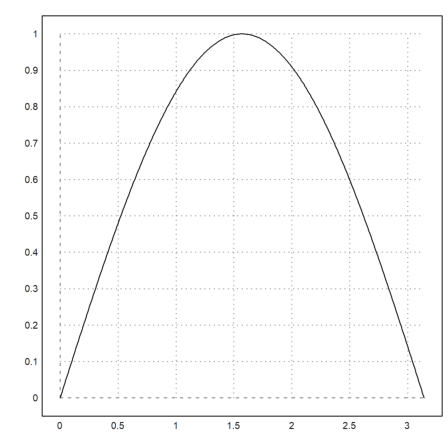
\includegraphics[keepaspectratio]{images/EMT4Kalkulus - Naila Khalidatus Salwa-342.png}}
\caption{images/EMT4Kalkulus\%20-\%20Naila\%20Khalidatus\%20Salwa-342.png}
\end{figure}

Carilah

\[\int_0^2 x^2 \sqrt{2x+1} dx\]\textgreater\$showev('integrate(x\^{}2*sqrt(2*x+1),x))

\[\int {x^2\,\sqrt{2\,x+1}}{\;dx}=\frac{\left(2\,x+1\right)^{\frac{7  }{2}}}{28}-\frac{\left(2\,x+1\right)^{\frac{5}{2}}}{10}+\frac{\left(  2\,x+1\right)^{\frac{3}{2}}}{12}\]\textgreater\$showev('integrate(x\^{}2*sqrt(2*x+1),x,0,2))

\[\int_{0}^{2}{x^2\,\sqrt{2\,x+1}\;dx}=\frac{2\,5^{\frac{5}{2}}}{21}-  \frac{2}{105}\]\textgreater\$ratsimp(\%)

\[\int_{0}^{2}{x^2\,\sqrt{2\,x+1}\;dx}=\frac{2\,5^{\frac{7}{2}}-2}{  105}\]\textgreater\$showev('integrate((sin(sqrt(x)+a)*E\textsuperscript{sqrt(x))/sqrt(x),x,0,pi}2))

\[\int_{0}^{\pi^2}{\frac{\sin \left(\sqrt{x}+a\right)\,e^{\sqrt{x}}}{  \sqrt{x}}\;dx}=\left(-e^{\pi}-1\right)\,\sin a+\left(e^{\pi}+1  \right)\,\cos a\]\textgreater\$factor(\%)

\[\int_{0}^{\pi^2}{\frac{\sin \left(\sqrt{x}+a\right)\,e^{\sqrt{x}}}{  \sqrt{x}}\;dx}=\left(-e^{\pi}-1\right)\,\left(\sin a-\cos a\right)\]\textgreater function map f(x) \&= E\textsuperscript{(-x}2)

\begin{verbatim}
                                    2
                                 - x
                                E
\end{verbatim}

\textgreater\$showev('integrate(f(x),x))

\[\int {e^ {- x^2 }}{\;dx}=\frac{\sqrt{\pi}\,\mathrm{erf}\left(x  \right)}{2}\]Fungsi f tidak memiliki antiturunan, integralnya masih memuat integral lain.

\[erf(x) = \int \frac{e^{-x^2}}{\sqrt{\pi}} \ dx.\]Kita tidak dapat menggunakan teorema Dasar kalkulus untuk menghitung integral tentu fungsi tersebut jika semua batasnya berhingga. Dalam hal ini dapat digunakan metode numerik (rumus kuadratur).

Misalkan kita akan menghitung:

\[\int_{0}^{\pi}{e^ {- x^2 }\;dx}\]\textgreater x=0:0.1:pi-0.1; plot2d(x,f(x+0.1),\textgreater bar); plot2d(``f(x)'',0,pi,\textgreater add):

\begin{figure}
\centering
\pandocbounded{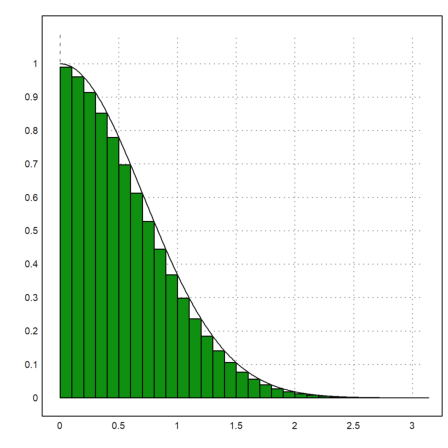
\includegraphics[keepaspectratio]{images/EMT4Kalkulus - Naila Khalidatus Salwa-352.png}}
\caption{images/EMT4Kalkulus\%20-\%20Naila\%20Khalidatus\%20Salwa-352.png}
\end{figure}

Integral tentu

\[\int_{0}^{\pi}{e^ {- x^2 }\;dx}\]dapat dihampiri dengan jumlah luas persegi-persegi panjang di bawah kurva y=f(x) tersebut. Langkah-langkahnya adalah sebagai berikut.

\textgreater t \&= makelist(a,a,0,pi-0.1,0.1);

mendefinisikan t sebagai list untuk menyimpan nilai-nilai x

\textgreater fx \&= makelist(f(t{[}i{]}+0.1),i,1,length(t));

simpan nilai-nilai f(x) dan jangan menggunakan x sebagai list

Hasilnya adalah:

\[\int_{0}^{\pi}{e^ {- x^2 }\;dx}=0.1950839272901491\]Jumlah tersebut diperoleh dari hasil kali lebar sub-subinterval (=0.1) dan jumlah nilai-nilai f(x) untuk x = 0.1, 0.2, 0.3, \ldots, 3.2.

\textgreater0.1*sum(f(x+0.1))

\begin{verbatim}
0.836219610253
\end{verbatim}

Untuk mendapatkan nilai integral tentu yang mendekati nilai sebenarnya, lebar sub-intervalnya dapat diperkecil lagi, sehingga daerah di bawah kurva tertutup semuanya, misalnya dapat digunakan lebar subinterval 0.001.

\textgreater x=0:0.001:pi-0.1; plot2d(x,f(x+0.1),\textgreater bar); plot2d(``f(x)'',0,pi,\textgreater add):

\begin{figure}
\centering
\pandocbounded{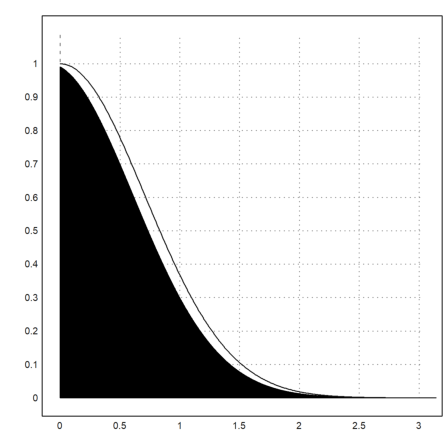
\includegraphics[keepaspectratio]{images/EMT4Kalkulus - Naila Khalidatus Salwa-355.png}}
\caption{images/EMT4Kalkulus\%20-\%20Naila\%20Khalidatus\%20Salwa-355.png}
\end{figure}

Berikut adalah contoh lain fungsi yang tidak memiliki antiderivatif, sehingga integral tentunya hanya dapat dihitung dengan metode numerik.

\textgreater function f(x) \&= x\^{}x

\begin{verbatim}
                                   x
                                  x
\end{verbatim}

\textgreater\$showev('integrate(f(x),x,0,1))

\[\int_{0}^{1}{x^{x}\;dx}=\int_{0}^{1}{x^{x}\;dx}\]\textgreater x=0:0.1:1-0.01; plot2d(x,f(x+0.01),\textgreater bar); plot2d(``f(x)'',0,1,\textgreater add):

\begin{figure}
\centering
\pandocbounded{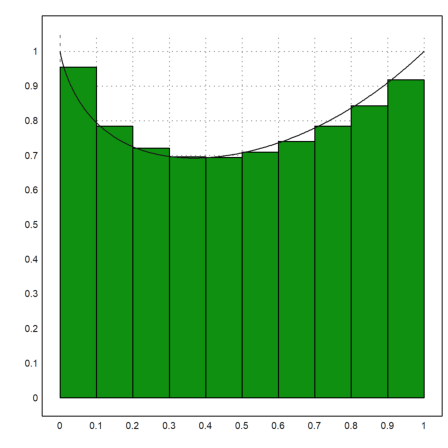
\includegraphics[keepaspectratio]{images/EMT4Kalkulus - Naila Khalidatus Salwa-357.png}}
\caption{images/EMT4Kalkulus\%20-\%20Naila\%20Khalidatus\%20Salwa-357.png}
\end{figure}

Karena maxima gagal menghitung integral tentu tersebut secara langsung menggunakan perintah integrate. Untuk mendapat hasil atau pendekatan nilai integral tentu tersebut kita lakukan seperti contoh sebelumnya.

\textgreater t \&= makelist(a,a,0,1-0.01,0.01);

\textgreater fx \&= makelist(f(t{[}i{]}+0.01),i,1,length(t));

\[\int_{0}^{1}{\sin ^2\left(3\,x^5+7\right)\;dx}=0.7834935879025506\]\textgreater function f(x) \&= sin(3*x\textsuperscript{5+7)}2; \$f(x)

\[\sin ^2\left(3\,x^5+7\right)\]\textgreater integrate(f,0,1)

\begin{verbatim}
0.542581176074
\end{verbatim}

\section{Sifat - Sifat Integral Tentu}\label{sifat---sifat-integral-tentu}

\begin{enumerate}
\def\labelenumi{\arabic{enumi}.}
\tightlist
\item
  Linearitas
\end{enumerate}

sifat 1: Jika c adalah konstanta, maka:

\[\int_a^b c f(x) dx = c \int_a^b f(x) dx\]

Sifat 2: Jika f(x) dan g(x) adalah dua fungsi yang terintegralkan pada interval {[}a, b{]}, maka:

\[\int_a^b (f(x) + g(x)) dx = \int_a^b f(x) dx + \int_a^b g(x) dx\]2. Interval

Sifat 3: Jika a \textless{} c \textless{} b, maka:

\[\int_a^b f(x) dx = \int_a^c f(x) dx + \int_c^b f(x) dx\]3. Fungsi Genap dan Ganjil

Fungsi Genap: Jika f(x) adalah fungsi genap (yaitu, f(-x) = f(x)), maka:

\[\int_{-a}^a f(x) dx = 2 \int_0^a f(x) dx\]

Fungsi Ganjil: Jika f(x) adalah fungsi ganjil (yaitu, f(-x) = -f(x)), maka:

\[\int_{-a}^a f(x) dx = 0\]4. Batas Integral Bertukar

\[\int_b^a f(x) dx = -\int_a^b f(x) dx\]\textgreater{}

\section{Aplikasi Integral Tentu}\label{aplikasi-integral-tentu}

\section{Aplikasi Integral Tentu pada Panjang Kurva}\label{aplikasi-integral-tentu-pada-panjang-kurva}

Sebuah jalan tol memiliki bentuk lengkungan yang dapat dimodelkan dengan persamaan y = x\^{}2 dari titik x = 0 hingga x = 2 (dalam kilometer). Berapakah panjang jalan tol tersebut

Penyelesaian:

\[s = \int_0^2 \sqrt{1 + (2x)^2} dx\]\textgreater\$showev('integrate(sqrt(1 + (2*x)\^{}2),x,0,2))

\[\int_{0}^{2}{\sqrt{4\,x^2+1}\;dx}=\frac{{\rm asinh}\; 4+4\,\sqrt{17  }}{4}\]\textgreater\$float(\%)

\[\int_{0.0}^{2.0}{\sqrt{4.0\,x^2+1.0}\;dx}=4.646783762432936\]Hitunglah panjang kurva berikut ini dan luas daerah di dalam kurva tersebut.

\[\gamma(t) = (r(t) \cos(t), r(t) \sin(t))\]dengan

\[r(t) = 1 + \dfrac{\sin(3t)}{2},\quad 0\le t\le 2\pi.\]\textgreater t=linspace(0,2pi,1000); r=1+sin(3*t)/2; x=r*cos(t); y=r*sin(t); \ldots{}\\
\textgreater{} plot2d(x,y,\textgreater filled,fillcolor=red,style=``/'',r=1.5): // Kita gambar kurvanya terlebih dahulu

\begin{figure}
\centering
\pandocbounded{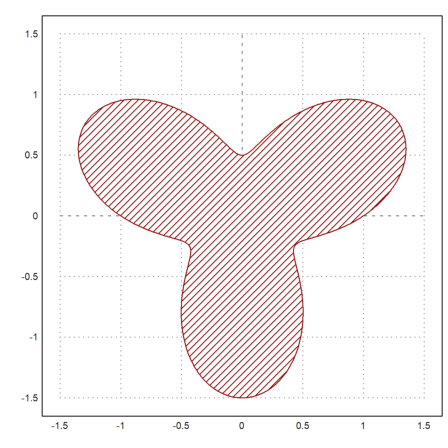
\includegraphics[keepaspectratio]{images/EMT4Kalkulus - Naila Khalidatus Salwa-371.png}}
\caption{images/EMT4Kalkulus\%20-\%20Naila\%20Khalidatus\%20Salwa-371.png}
\end{figure}

\textgreater function r(t) \&= 1+sin(3*t)/2; \$'r(t)=r(t)

\[r\left(t\right)=\frac{\sin \left(3\,t\right)}{2}+1\]\textgreater function fx(t) \&= r(t)*cos(t); \$'fx(t)=fx(t)

\[{\it fx}\left(t\right)=\cos t\,\left(\frac{\sin \left(3\,t\right)}{  2}+1\right)\]\textgreater function fy(t) \&= r(t)*sin(t); \$'fy(t)=fy(t)

\[{\it fy}\left(t\right)=\sin t\,\left(\frac{\sin \left(3\,t\right)}{  2}+1\right)\]\textgreater function ds(t) \&= trigreduce(radcan(sqrt(diff(fx(t),t)\textsuperscript{2+diff(fy(t),t)}2))); \$'ds(t)=ds(t)

\[{\it ds}\left(t\right)=\frac{\sqrt{4\,\cos \left(6\,t\right)+4\,  \sin \left(3\,t\right)+9}}{2}\]\textgreater\$integrate(ds(x),x,0,2*pi) //panjang (keliling) kurva

\[\frac{\int_{0}^{2\,\pi}{\sqrt{4\,\cos \left(6\,x\right)+4\,\sin   \left(3\,x\right)+9}\;dx}}{2}\]Maxima gagal melakukan perhitungan eksak integral tersebut.

Berikut kita hitung integralnya secara numerik dengan perintah EMT.

\textgreater integrate(``ds(x)'',0,2*pi)

\begin{verbatim}
9.0749467823
\end{verbatim}

Spiral Logaritmik

\[x=e^{ax}\cos x,\ y=e^{ax}\sin x.\]\textgreater a=0.1; plot2d(``exp(a*x)*cos(x)'',``exp(a*x)*sin(x)'',r=2,xmin=0,xmax=2*pi):

\begin{figure}
\centering
\pandocbounded{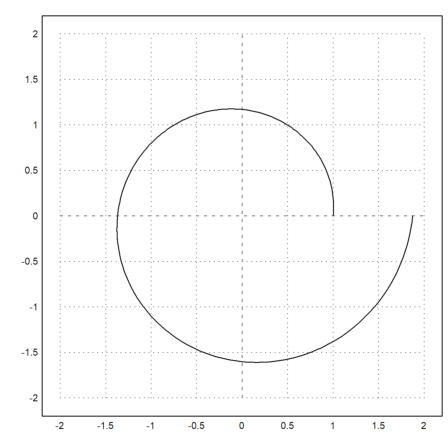
\includegraphics[keepaspectratio]{images/EMT4Kalkulus - Naila Khalidatus Salwa-378.png}}
\caption{images/EMT4Kalkulus\%20-\%20Naila\%20Khalidatus\%20Salwa-378.png}
\end{figure}

\textgreater\&kill(a) // hapus expresi a

\begin{verbatim}
                                 done
\end{verbatim}

\textgreater function fx(t) \&= exp(a*t)*cos(t); \$'fx(t)=fx(t)

\[{\it fx}\left(t\right)=e^{a\,t}\,\cos t\]\textgreater function fy(t) \&= exp(a*t)*sin(t); \$'fy(t)=fy(t)

\[{\it fy}\left(t\right)=e^{a\,t}\,\sin t\]\textgreater function df(t) \&= trigreduce(radcan(sqrt(diff(fx(t),t)\textsuperscript{2+diff(fy(t),t)}2))); \$'df(t)=df(t)

\[{\it df}\left(t\right)=\sqrt{a^2+1}\,e^{a\,t}\]\textgreater S \&=integrate(df(t),t,0,2*\%pi); \$S // panjang kurva (spiral)

\[\sqrt{a^2+1}\,\left(\frac{e^{2\,\pi\,a}}{a}-\frac{1}{a}\right)\]\textgreater S(a=0.1) // Panjang kurva untuk a=0.1

\begin{verbatim}
8.78817491636
\end{verbatim}

Soal:

Tunjukkan bahwa keliling lingkaran dengan jari-jari r adalah K=2.pi.r.

Penyelesaian:

Lingkaran dalam Koordinat Kartesius: Kita dapat merepresentasikan suatu lingkaran dengan pusat di titik asal (0,0) dan jari-jari r dengan persamaan parametrik berikut:

\[x(t) = r \cos(t)\]\[y(t) = r \sin(t)\]

di mana t adalah parameter yang bervariasi dari 0 hingga 2p.

Panjang Kurva Parametrik: Panjang kurva parametrik (x(t), y(t)) dari t=a hingga t=b dapat dihitung dengan integral:

\[s = \int_a^b \sqrt{\left(\frac{dx}{dt}\right)^2 + \left(\frac{dy}{dt}\right)^2} dt\]1. Mencari Turunan

\[x(t) = r \cos(t)\]\textgreater\&showev('diff(r*cos(t),t))

\begin{verbatim}
                      d
                      -- (r cos(t)) = - r sin(t)
                      dt
\end{verbatim}

\[y(t)=rsin(t)\]\textgreater\&showev('diff(r*sin(t),t))

\begin{verbatim}
                       d
                       -- (r sin(t)) = r cos(t)
                       dt
\end{verbatim}

\begin{enumerate}
\def\labelenumi{\arabic{enumi}.}
\setcounter{enumi}{1}
\tightlist
\item
  Substitusi ke Rumus Panjang Kurva:
\end{enumerate}

\[s = \int_0^{2\pi} \sqrt{(-r \sin(t))^2 + (r \cos(t))^2} dt\]\[s = \int_0^{2\pi} \sqrt{r^2 (\sin^2(t) + \cos^2(t))} dt\]

Karena

\[sin^2(t) + cos^2(t) = 1,\]

maka:

\[s = \int_0^{2\pi} r dt\]3. Integral

\[s = r \int_0^{2\pi} dt = r[t]_0^{2\pi} = r(2p - 0) = 2\pi r\]Berikut adalah contoh menghitung panjang parabola.

\textgreater plot2d(``x\^{}2'',xmin=-1,xmax=1):

\begin{figure}
\centering
\pandocbounded{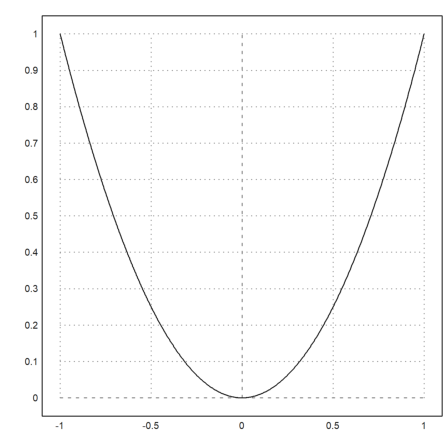
\includegraphics[keepaspectratio]{images/EMT4Kalkulus - Naila Khalidatus Salwa-393.png}}
\caption{images/EMT4Kalkulus\%20-\%20Naila\%20Khalidatus\%20Salwa-393.png}
\end{figure}

\textgreater\$showev('integrate(sqrt(1+diff(x\textsuperscript{2,x)}2),x,-1,1))

\[\int_{-1}^{1}{\sqrt{4\,x^2+1}\;dx}=\frac{{\rm asinh}\; 2+2\,\sqrt{5  }}{2}\]\textgreater\$float(\%)

\[\int_{-1.0}^{1.0}{\sqrt{4.0\,x^2+1.0}\;dx}=2.957885715089195\]\textgreater x=-1:0.2:1; y=x\^{}2; plot2d(x,y); \ldots{}\\
\textgreater{} plot2d(x,y,points=1,style=``o\#'',add=1):

\begin{figure}
\centering
\pandocbounded{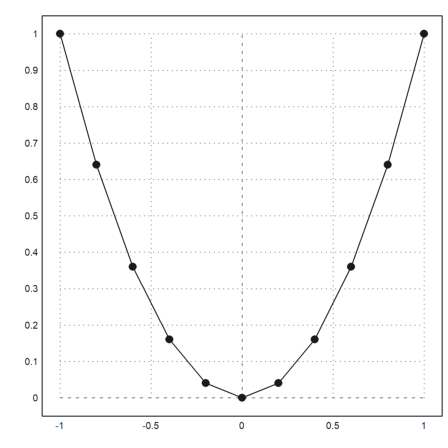
\includegraphics[keepaspectratio]{images/EMT4Kalkulus - Naila Khalidatus Salwa-396.png}}
\caption{images/EMT4Kalkulus\%20-\%20Naila\%20Khalidatus\%20Salwa-396.png}
\end{figure}

Panjang tersebut dapat dihampiri dengan menggunakan jumlah panjang ruas-ruas garis yang menghubungkan titik-titik pada parabola tersebut.

\textgreater i=1:cols(x)-1; sum(sqrt((x{[}i+1{]}-x{[}i{]})\textsuperscript{2+(y{[}i+1{]}-y{[}i{]})}2))

\begin{verbatim}
2.95191957027
\end{verbatim}

Hasilnya mendekati panjang yang dihitung secara eksak. Untuk mendapatkan hampiran yang cukup akurat, jarak antar titik dapat diperkecil, misalnya 0.1, 0.05, 0.01, dan seterusnya. Cobalah Anda ulangi perhitungannya dengan nilai-nilai tersebut.

\section{Koordinat Kartesius}\label{koordinat-kartesius}

Berikut diberikan contoh perhitungan panjang kurva menggunakan koordinat Kartesius. Kita akan hitung panjang kurva dengan persamaan implisit:

\[x^3+y^3-3xy=0.\]\textgreater z \&= x\textsuperscript{3+y}3-3*x*y; \$z

\[y^3-3\,x\,y+x^3\]\textgreater plot2d(z,r=2,level=0,n=100):

\begin{figure}
\centering
\pandocbounded{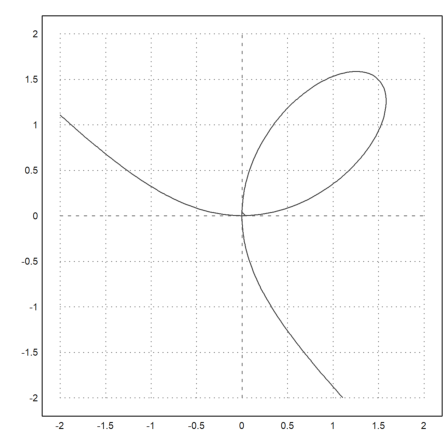
\includegraphics[keepaspectratio]{images/EMT4Kalkulus - Naila Khalidatus Salwa-399.png}}
\caption{images/EMT4Kalkulus\%20-\%20Naila\%20Khalidatus\%20Salwa-399.png}
\end{figure}

Kita tertarik pada kurva di kuadran pertama.

\textgreater plot2d(z,a=0,b=2,c=0,d=2,level={[}-10;0{]},n=100,contourwidth=3,style=``/''):

\begin{figure}
\centering
\pandocbounded{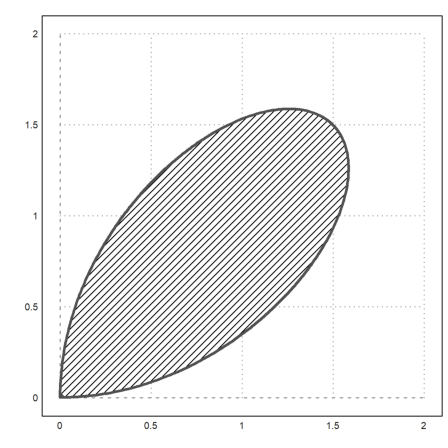
\includegraphics[keepaspectratio]{images/EMT4Kalkulus - Naila Khalidatus Salwa-400.png}}
\caption{images/EMT4Kalkulus\%20-\%20Naila\%20Khalidatus\%20Salwa-400.png}
\end{figure}

\textgreater plot2d(z,a=0,b=2,c=0,d=2,level={[}-10;0{]},n=100,contourwidth=3,style=``/''):

\begin{figure}
\centering
\pandocbounded{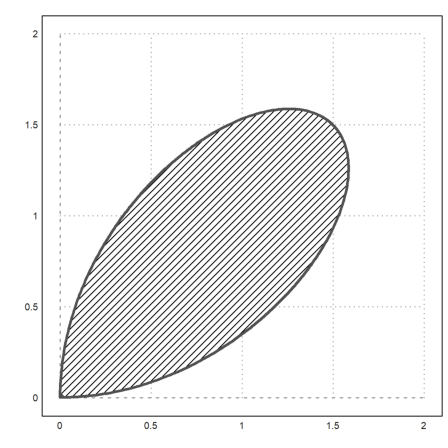
\includegraphics[keepaspectratio]{images/EMT4Kalkulus - Naila Khalidatus Salwa-401.png}}
\caption{images/EMT4Kalkulus\%20-\%20Naila\%20Khalidatus\%20Salwa-401.png}
\end{figure}

Kita selesaikan persamaannya untuk x.

\textgreater\$z with y=l*x, sol \&= solve(\%,x); \$sol

\[\left[ x=\frac{3\,l}{l^3+1} , x=0 \right] \]\pandocbounded{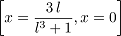
\includegraphics[keepaspectratio]{images/EMT4Kalkulus - Naila Khalidatus Salwa-403.png}}

Kita gunakan solusi tersebut untuk mendefinisikan fungsi dengan Maxima.

\textgreater function f(l) \&= rhs(sol{[}1{]}); \$'f(l)=f(l)

\[f\left(l\right)=\frac{3\,l}{l^3+1}\]Fungsi tersebut juga dapat digunaka untuk menggambar kurvanya. Ingat, bahwa fungsi tersebut adalah nilai x dan nilai y=l\emph{x, yakni x=f(l) dan y=l}f(l).

\textgreater plot2d(\&f(x),\&x*f(x),xmin=-0.5,xmax=2,a=0,b=2,c=0,d=2,r=1.5):

\begin{figure}
\centering
\pandocbounded{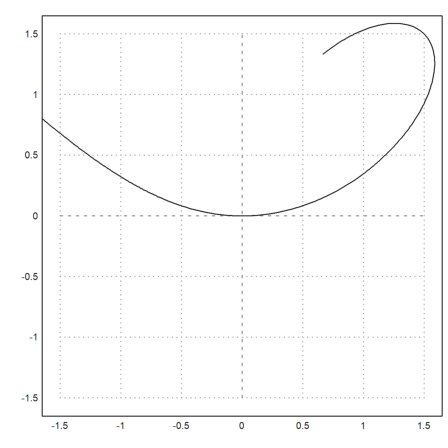
\includegraphics[keepaspectratio]{images/EMT4Kalkulus - Naila Khalidatus Salwa-405.png}}
\caption{images/EMT4Kalkulus\%20-\%20Naila\%20Khalidatus\%20Salwa-405.png}
\end{figure}

Elemen panjang kurva adalah:

\[ds=\sqrt{f'(l)^2+(lf'(l)+f(l))^2}.\]\textgreater function ds(l) \&= ratsimp(sqrt(diff(f(l),l)\textsuperscript{2+diff(l*f(l),l)}2)); \$'ds(l)=ds(l)

\[{\it ds}\left(l\right)=\frac{\sqrt{9\,l^8+36\,l^6-36\,l^5-36\,l^3+  36\,l^2+9}}{\sqrt{l^{12}+4\,l^9+6\,l^6+4\,l^3+1}}\]\textgreater\$integrate(ds(l),l,0,1)

\[\int_{0}^{1}{\frac{\sqrt{9\,l^8+36\,l^6-36\,l^5-36\,l^3+36\,l^2+9}  }{\sqrt{l^{12}+4\,l^9+6\,l^6+4\,l^3+1}}\;dl}\]Integral tersebut tidak dapat dihitung secara eksak menggunakan Maxima. Kita hitung integral etrsebut secara numerik dengan Euler. Karena kurva simetris, kita hitung untuk nilai variabel integrasi dari 0 sampai 1, kemudian hasilnya dikalikan 2.

\textgreater2*integrate(``ds(x)'',0,1)

\begin{verbatim}
4.91748872168
\end{verbatim}

\textgreater2*romberg(\&ds(x),0,1)// perintah Euler lain untuk menghitung nilai hampiran integral

\begin{verbatim}
4.91748872168
\end{verbatim}

Perhitungan di atas dapat dilakukan untuk sebarang fungsi x dan y dengan mendefinisikan fungsi EMT, misalnya kita beri nama panjangkurva. Fungsi ini selalu memanggil Maxima untuk menurunkan fungsi yang diberikan.

\textgreater function panjangkurva(fx,fy,a,b) \ldots{}

\begin{verbatim}
ds=mxm("sqrt(diff(@fx,x)^2+diff(@fy,x)^2)");
return romberg(ds,a,b);
endfunction
\end{verbatim}

\textgreater panjangkurva(``x'',``x\^{}2'',-1,1)

\begin{verbatim}
2.95788571509
\end{verbatim}

Bandingkan dengan nilai eksak di atas.

\textgreater2*panjangkurva(mxm(``f(x)''),mxm(``x*f(x)''),0,1)

\begin{verbatim}
4.91748872168
\end{verbatim}

Kita hitung panjang spiral Archimides berikut ini dengan fungsi tersebut.

\textgreater plot2d(``x*cos(x)'',``x*sin(x)'',xmin=0,xmax=2*pi,square=1):

\begin{figure}
\centering
\pandocbounded{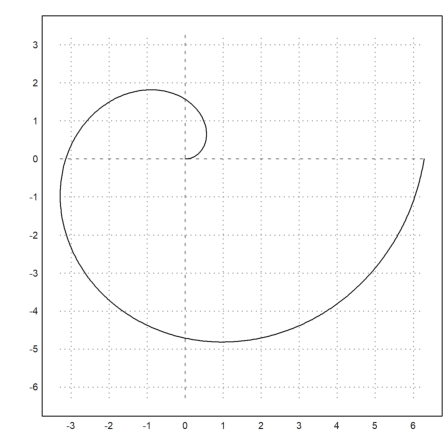
\includegraphics[keepaspectratio]{images/EMT4Kalkulus - Naila Khalidatus Salwa-409.png}}
\caption{images/EMT4Kalkulus\%20-\%20Naila\%20Khalidatus\%20Salwa-409.png}
\end{figure}

\textgreater panjangkurva(``x*cos(x)'',``x*sin(x)'',0,2*pi)

\begin{verbatim}
21.2562941482
\end{verbatim}

Berikut kita definisikan fungsi yang sama namun dengan Maxima, untuk perhitungan eksak.

\textgreater\&kill(ds,x,fx,fy)

\begin{verbatim}
                                 done
\end{verbatim}

\textgreater function ds(fx,fy) \&\&= sqrt(diff(fx,x)\textsuperscript{2+diff(fy,x)}2)

\begin{verbatim}
                           2              2
                  sqrt(diff (fy, x) + diff (fx, x))
\end{verbatim}

\textgreater sol \&= ds(x*cos(x),x*sin(x)); \$sol // Kita gunakan untuk menghitung panjang kurva terak

\[\sqrt{\left(\cos x-x\,\sin x\right)^2+\left(\sin x+x\,\cos x\right)  ^2}\]\textgreater\$sol \textbar{} trigreduce \textbar{} expand, \$integrate(\%,x,0,2*pi), \%()

\[\frac{{\rm asinh}\; \left(2\,\pi\right)+2\,\pi\,\sqrt{4\,\pi^2+1}}{  2}\]\pandocbounded{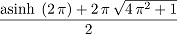
\includegraphics[keepaspectratio]{images/EMT4Kalkulus - Naila Khalidatus Salwa-412.png}}

\begin{verbatim}
21.2562941482
\end{verbatim}

Hasilnya sama dengan perhitungan menggunakan fungsi EMT.

Berikut adalah contoh lain penggunaan fungsi Maxima tersebut.

\textgreater plot2d(``3*x\textsuperscript{2-1'',''3*x}3-1'',xmin=-1/sqrt(3),xmax=1/sqrt(3),square=1):

\begin{figure}
\centering
\pandocbounded{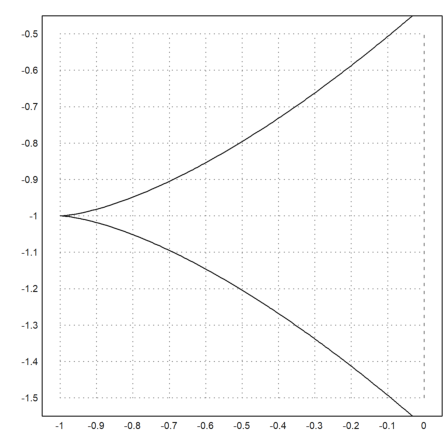
\includegraphics[keepaspectratio]{images/EMT4Kalkulus - Naila Khalidatus Salwa-413.png}}
\caption{images/EMT4Kalkulus\%20-\%20Naila\%20Khalidatus\%20Salwa-413.png}
\end{figure}

\textgreater sol \&= radcan(ds(3*x\textsuperscript{2-1,3*x}3-1)); \$sol

\[3\,x\,\sqrt{9\,x^2+4}\]\textgreater\$showev('integrate(sol,x,0,1/sqrt(3))), \$2*float(\%) // panjang kurva di atas

\[6.0\,\int_{0.0}^{0.5773502691896258}{x\,\sqrt{9.0\,x^2+4.0}\;dx}=  2.337835372767141\]\pandocbounded{\includegraphics[keepaspectratio]{images/EMT4Kalkulus - Naila Khalidatus Salwa-416.png}}

\section{Sikloid}\label{sikloid}

Berikut kita akan menghitung panjang kurva lintasan (sikloid) suatu titik pada lingkaran yang berputar ke kanan pada permukaan datar. Misalkan jari-jari lingkaran tersebut adalah r. Posisi titik pusat lingkaran pada saat t adalah:

\[(rt,r).\]Misalkan posisi titik pada lingkaran tersebut mula-mula (0,0) dan posisinya pada saat t adalah:

\[(r(t-\sin(t)),r(1-\cos(t))).\]Berikut kita plot lintasan tersebut dan beberapa posisi lingkaran ketika t=0, t=pi/2, t=r*pi.

\textgreater x \&= r*(t-sin(t))

\begin{verbatim}
                            r (t - sin(t))
\end{verbatim}

\textgreater y \&= r*(1-cos(t))

\begin{verbatim}
                            r (1 - cos(t))
\end{verbatim}

Berikut kita gambar sikloid untuk r=1.

\textgreater{} ex \&= x-sin(x); ey \&= 1-cos(x); aspect(1);

\textgreater plot2d(ex,ey,xmin=0,xmax=4pi,square=1); \ldots{}\\
\textgreater{} plot2d(``2+cos(x)'',``1+sin(x)'',xmin=0,xmax=2pi,\textgreater add,color=blue); \ldots{}\\
\textgreater{} plot2d({[}2,ex(2){]},{[}1,ey(2){]},color=red,\textgreater add); \ldots{}\\
\textgreater{} plot2d(ex(2),ey(2),\textgreater points,\textgreater add,color=red); \ldots{}\\
\textgreater{} plot2d(``2pi+cos(x)'',``1+sin(x)'',xmin=0,xmax=2pi,\textgreater add,color=blue); \ldots{}\\
\textgreater{} plot2d({[}2pi,ex(2pi){]},{[}1,ey(2pi){]},color=red,\textgreater add); \ldots{}\\
\textgreater{} plot2d(ex(2pi),ey(2pi),\textgreater points,\textgreater add,color=red):

\begin{figure}
\centering
\pandocbounded{\includegraphics[keepaspectratio]{images/EMT4Kalkulus - Naila Khalidatus Salwa-419.png}}
\caption{images/EMT4Kalkulus\%20-\%20Naila\%20Khalidatus\%20Salwa-419.png}
\end{figure}

Berikut dihitung panjang lintasan untuk 1 putaran penuh. (Jangan salah menduga bahwa panjang lintasan 1 putaran penuh sama dengan keliling lingkaran!)

\textgreater ds \&= radcan(sqrt(diff(ex,x)\textsuperscript{2+diff(ey,x)}2)); \$ds=trigsimp(ds) // elemen panjang kurva sikloid

\[\sqrt{\sin ^2x+\cos ^2x-2\,\cos x+1}=\sqrt{2-2\,\cos x}\]\textgreater ds \&= trigsimp(ds); \$ds

\[\sqrt{2-2\,\cos x}\]\textgreater\$showev('integrate(ds,x,0,2*pi)) // hitung panjang sikloid satu putaran penuh

\[\int_{0}^{2\,\pi}{\sqrt{2-2\,\cos x}\;dx}=8\]\textgreater integrate(mxm(``ds''),0,2*pi) // hitung secara numerik

\begin{verbatim}
8
\end{verbatim}

\textgreater romberg(mxm(``ds''),0,2*pi) // cara lain hitung secara numerik

\begin{verbatim}
8
\end{verbatim}

Perhatikan, seperti terlihat pada gambar, panjang sikloid lebih besar daripada keliling lingkarannya, yakni:

\[2\pi.\]\#\# Kurvatur (Kelengkungan) Kurva

\begin{figure}
\centering
\pandocbounded{\includegraphics[keepaspectratio]{images/EMT4Kalkulus - Naila Khalidatus Salwa-424.png}}
\caption{images/EMT4Kalkulus\%20-\%20Naila\%20Khalidatus\%20Salwa-424.png}
\end{figure}

Aslinya, kelengkungan kurva diferensiabel (yakni, kurva mulus yang tidak lancip) di titik P didefinisikan melalui lingkaran oskulasi (yaitu, lingkaran yang melalui titik P dan terbaik memperkirakan, paling banyak menyinggung kurva di sekitar P). Pusat dan radius kelengkungan kurva di P adalah pusat dan radius lingkaran oskulasi. Kelengkungan adalah kebalikan dari radius kelengkungan:

\[\kappa =\frac {1}{R}\]dengan R adalah radius kelengkungan. (Setiap lingkaran memiliki kelengkungan ini pada setiap titiknya, dapat diartikan, setiap lingkaran berputar 2pi sejauh 2piR.)

Definisi ini sulit dimanipulasi dan dinyatakan ke dalam rumus untuk kurva umum. Oleh karena itu digunakan definisi lain yang ekivalen.

\chapter{6. Barisan dan Deret}\label{barisan-dan-deret}

Barisan adalah susunan bilangan yang memiliki pola atau karakteristik tertentu, sedangkan deret adalah hasil penjumlahan dari anggota-anggota dalam barian tertentu.

Barisan dapat didefinisikan dengan beberapa cara di dalam EMT, di antaranya:

\begin{itemize}
\item
  menggunakan titik dua ``:'', sama seperti saat mendefinisikan vektor dengan elemen-elemen beraturan
\item
  menggunakan perintah ``sequence'' dan rumus barisan (suku ke -n);
\item
  menggunakan perintah ``iterate'' atau ``niterate'';
\item
  menggunakan fungsi Maxima ``create\_list'' atau ``makelist'' untuk menghasilkan barisan simbolik;
\item
  menggunakan fungsi biasa yang inputnya vektor atau barisan;
\item
  menggunakan fungsi rekursif.
\end{itemize}

EMT menyediakan beberapa perintah (fungsi) terkait barisan, yakni:

\begin{itemize}
\item
  sum: menghitung jumlah semua elemen suatu barisan
\item
  cumsum: jumlah kumulatif suatu barisan
\item
  differences: selisih antar elemen-elemen berturutan
\end{itemize}

EMT juga dapat digunakan untuk menghitung jumlah deret berhingga maupun deret tak hingga, dengan menggunakan perintah (fungsi) ``sum''. Perhitungan dapat dilakukan secara numerik maupun simbolik dan eksak.

Contoh perhitungan barisan dan deret menggunakan EMT.

\section{Menggunakan titik dua}\label{menggunakan-titik-dua}

\textgreater1:15

\begin{verbatim}
[1,  2,  3,  4,  5,  6,  7,  8,  9,  10,  11,  12,  13,  14,  15]
\end{verbatim}

\textgreater1:3:30

\begin{verbatim}
[1,  4,  7,  10,  13,  16,  19,  22,  25,  28]
\end{verbatim}

\textgreater sum(1:3:30)

\begin{verbatim}
145
\end{verbatim}

\textgreater cumsum(1:3:30)

\begin{verbatim}
[1,  5,  12,  22,  35,  51,  70,  92,  117,  145]
\end{verbatim}

\section{Menggunakan perintah ``sequence'' dan rumus barisan (suku ke -n)}\label{menggunakan-perintah-sequence-dan-rumus-barisan-suku-ke--n}

Untuk barisan yang lebih kompleks dapat digunakan fungsi ``sequence()''. Fungsi ini menghitung nilai-nilai x{[}n{]} dari semua nilai sebelumnya, x{[}1{]},\ldots,x{[}n-1{]} yang diketahui.

Berikut adalah contoh barisan Fibonacci.

\[x_n = x_{n-1}+x_{n-2}, \quad x_1=1, \quad x_2 =1\]\textgreater sequence(``x{[}n-1{]}+x{[}n-2{]}'',{[}1,1{]},15) //suku ke satu :1, suku ke dua :1

\begin{verbatim}
[1,  1,  2,  3,  5,  8,  13,  21,  34,  55,  89,  144,  233,  377,  610]
\end{verbatim}

\textgreater plot2d(sequence(``x{[}n-1{]}+x{[}n-2{]}'',{[}1,1{]},15)):

\begin{figure}
\centering
\pandocbounded{\includegraphics[keepaspectratio]{images/EMT4Kalkulus - Naila Khalidatus Salwa-427.png}}
\caption{images/EMT4Kalkulus\%20-\%20Naila\%20Khalidatus\%20Salwa-427.png}
\end{figure}

\textgreater sequence(``x{[}n-1{]}+x{[}n-2{]}'',{[}1,1{]},250)\^{}(1/(1:250))

\begin{verbatim}
[1,  1,  1.25992,  1.31607,  1.37973,  1.41421,  1.44256,  1.46311,
1.47967,  1.49292,  1.50389,  1.51309,  1.52091,  1.52765,  1.53352,
1.53867,  1.54323,  1.54729,  1.55094,  1.55422,  1.5572,  1.55992,
1.5624,  1.56468,  1.56678,  1.56872,  1.57052,  1.57219,  1.57375,
1.57521,  1.57657,  1.57785,  1.57905,  1.58019,  1.58126,  1.58227,
1.58322,  1.58413,  1.58499,  1.58581,  1.58659,  1.58733,  1.58804,
1.58871,  1.58936,  1.58997,  1.59057,  1.59113,  1.59168,  1.5922,
1.5927,  1.59319,  1.59365,  1.5941,  1.59453,  1.59495,  1.59535,
1.59574,  1.59611,  1.59648,  1.59683,  1.59717,  1.5975,  1.59782,
1.59813,  1.59843,  1.59872,  1.599,  1.59927,  1.59954,  1.5998,
1.60005,  1.6003,  1.60053,  1.60077,  1.60099,  1.60121,  1.60143,
1.60164,  1.60184,  1.60204,  1.60223,  1.60242,  1.60261,  1.60279,
1.60296,  1.60314,  1.60331,  1.60347,  1.60363,  1.60379,  1.60394,
1.60409,  1.60424,  1.60439,  1.60453,  1.60467,  1.6048,  1.60494,
1.60507,  1.60519,  1.60532,  1.60544,  1.60556,  1.60568,  1.6058,
1.60591,  1.60602,  1.60613,  1.60624,  1.60635,  1.60645,  1.60655,
1.60665,  1.60675,  1.60685,  1.60694,  1.60704,  1.60713,  1.60722,
1.60731,  1.6074,  1.60748,  1.60757,  1.60765,  1.60773,  1.60781,
1.60789,  1.60797,  1.60805,  1.60813,  1.6082,  1.60827,  1.60835,
1.60842,  1.60849,  1.60856,  1.60863,  1.60869,  1.60876,  1.60883,
 ... ]
\end{verbatim}

\textgreater plot2d(sequence(``x{[}n-1{]}+x{[}n-2{]}'',{[}1,1{]},250)\^{}(1/(1:250))):

\begin{figure}
\centering
\pandocbounded{\includegraphics[keepaspectratio]{images/EMT4Kalkulus - Naila Khalidatus Salwa-428.png}}
\caption{images/EMT4Kalkulus\%20-\%20Naila\%20Khalidatus\%20Salwa-428.png}
\end{figure}

\section{Menggunakan perintah ``iterate'' atau ``niterate''}\label{menggunakan-perintah-iterate-atau-niterate}

EMT menyediakan fungsi iterate(``g(x)'', x0, n) untuk melakukan iterasi

\[x_{k+1}=g(x_k), \ x_0=x_0, k= 1, 2, 3, ..., n.\]Berikut contoh penggunaan iterasi

Contoh : Menunjukkan pertumbuhan dari nilai awal 1000 dengan laju pertambahan 5\%, selama 10 periode.

\textgreater q=1.05; iterate(``x*q'',1000,n=10)'

\begin{verbatim}
         1000 
         1050 
       1102.5 
      1157.63 
      1215.51 
      1276.28 
       1340.1 
       1407.1 
      1477.46 
      1551.33 
      1628.89 
\end{verbatim}

\chapter{Spiral Theodorus}\label{spiral-theodorus}

konstruksi segitiga siku-siku yang berkesinambungan menjadi spiral atau dalam kata lain sebuah spiral yang dibangun dari segitiga siku-siku yang berurutan. Setiap segitiga siku-siku yang baru dibuat dengan menghubungkan sisi miring segitiga sebelumnya dengan sisi alas yang panjangnya 1 satuan.

Spiral Theodorus (spiral segitiga siku-siku) dapat digambar secara rekursif. Rumus rekursifnya adalah:

\[x_n = \left( 1 + \frac{i}{\sqrt{n-1}} \right) \, x_{n-1}, \quad x_1=1,\]yang menghasilkan barisan bilangan kompleks.

\textgreater function g(n) := 1+I/sqrt(n)

Rekursinya dapat dijalankan sebanyak 17 untuk menghasilkan barisan 17 bilangan kompleks, kemudian digambar bilangan-bilangan kompleksnya.

\textgreater x=sequence(``g(n-1)*x{[}n-1{]}'',1,20); plot2d(x,r=3.5);\ldots{}\\
\textgreater{} textbox(latex(``Spiral\textbackslash{} Theodorus''),0.4):

\begin{figure}
\centering
\pandocbounded{\includegraphics[keepaspectratio]{images/EMT4Kalkulus - Naila Khalidatus Salwa-431.png}}
\caption{images/EMT4Kalkulus\%20-\%20Naila\%20Khalidatus\%20Salwa-431.png}
\end{figure}

Selanjutnya dihubungan titik 0 dengan titik-titik kompleks tersebut menggunakan loop.

\textgreater for i=1:cols(x); plot2d({[}0,x{[}i{]}{]},\textgreater add); end:

\begin{figure}
\centering
\pandocbounded{\includegraphics[keepaspectratio]{images/EMT4Kalkulus - Naila Khalidatus Salwa-432.png}}
\caption{images/EMT4Kalkulus\%20-\%20Naila\%20Khalidatus\%20Salwa-432.png}
\end{figure}

\textgreater function gstep (v) \ldots{}

\begin{verbatim}
w=[-v[2];v[1]];
return v+w/norm(w);
endfunction
\end{verbatim}

\textgreater x=iterate(``gstep'',{[}1;0{]},16); plot2d(x{[}1{]},x{[}2{]},r=3.5,\textgreater points):

\begin{figure}
\centering
\pandocbounded{\includegraphics[keepaspectratio]{images/EMT4Kalkulus - Naila Khalidatus Salwa-433.png}}
\caption{images/EMT4Kalkulus\%20-\%20Naila\%20Khalidatus\%20Salwa-433.png}
\end{figure}

\section{Limit Barisan}\label{limit-barisan}

Limit dari suatu barisan (x\_n) saat (n) mendekati tak hingga adalah nilai yang didekati oleh elemen-elemen barisan tersebut seiring dengan bertambahnya (n). Secara formal, kita mengatakan bahwa barisan (x\_n) memiliki limit (L).

Definisi formal:

\[\forall \varepsilon > 0, \exists k \in \mathbb{N} : (\forall n \in \mathbb{N}, n \geq k \implies |x_n - L| <\varepsilon)\]Dapat dinotasikan sebagai

\[\lim_{n \to \infty}x_n=L\]Contoh:

\begin{enumerate}
\def\labelenumi{\arabic{enumi}.}
\tightlist
\item
\end{enumerate}

\[x_n = \lim_{n \to \infty}\frac{1}{n}\]\textgreater\$showev('limit(1/n,n,inf))

\[\lim_{n\rightarrow \infty }{\frac{1}{n}}=0\]\textgreater\$x\_n := 1/n

\[\frac{1}{n}\]\textgreater\$limit(x\_n,n,inf)

\[0\]2.

\[\lim_{n\to\infty}\frac{2n^2-1}{n^2+5}\]\textgreater\$showev('limit((2*n\textsuperscript{2-1)/(n}2+5),n,inf))

\[\lim_{n\rightarrow \infty }{\frac{2\,n^2-1}{n^2+5}}=2\]\# Kekonvergenan

Iterasi sampai konvergen merupakan proses yang terus berulang sampai mendapat nilai yang stabil atau tidak berubah secara signifikan. Tetapi, apabila iterasinya tidak konvergen setelah ditunggu lama, Kita dapat menghentikannya dengan menekan tombol {[}ESC{]}.

\textgreater iterate(``cos(x)'',1) // iterasi x(n+1)=cos(x(n)), dengan x(0)=1.

\begin{verbatim}
0.739085133216
\end{verbatim}

Iterasi tersebut konvergen ke penyelesaian persamaan

\[x = \cos(x).\]Iterasi ini juga dapat dilakukan pada interval, hasilnya adalah barisan interval yang memuat akar tersebut.

\textgreater hasil := iterate(``cos(x)'',\textsubscript{1,2}) //iterasi x(n+1)=cos(x(n)), dengan interval awal (1, 2)

\begin{verbatim}
~0.739085133211,0.7390851332133~
\end{verbatim}

\textgreater h=expand(hasil,100), cos(h) \textless\textless{} h

\begin{verbatim}
~0.73908513309,0.73908513333~
1
\end{verbatim}

Iterasi juga dapat digunakan pada fungsi yang didefinisikan.

\textgreater function f(x) := (x+2/x)/2

Iterasi x(n+1)=f(x(n)) akan konvergen ke akar kuadrat 2.

\textgreater iterate(``f'',2), sqrt(2)

\begin{verbatim}
1.41421356237
1.41421356237
\end{verbatim}

\chapter{Deret Taylor}\label{deret-taylor}

Deret Taylor suatu fungsi f yang diferensiabel sampai tak hingga di sekitar x=a adalah:

\[f(x) = \sum_{k=0}^\infty \frac{(x-a)^k f^{(k)}(a)}{k!}.\]Diberikan contoh fungsi exponensial yang didekati dengan Deret Taylor

\textgreater{} \$'e\^{}x =taylor(exp(x),x,0,10)

\[e^{x}=\frac{x^{10}}{3628800}+\frac{x^9}{362880}+\frac{x^8}{40320}+  \frac{x^7}{5040}+\frac{x^6}{720}+\frac{x^5}{120}+\frac{x^4}{24}+  \frac{x^3}{6}+\frac{x^2}{2}+x+1\]\textgreater x := 4; k := 10; hasil := round(exp(x),k)

\begin{verbatim}
54.5981500331
\end{verbatim}

Bukti :

\[e^x = \frac{(x)^{10}}{(3628800)} + \frac{(x)^{9}}{(362880)} + \frac{(x)^{8}}{(40320)} + \frac{(x)^{7}}{(5040)} + \frac{(x)^{6}}{(720)} + \frac{(x)^{5}}{(120)} + \frac{(x)^{4}}{(24)} + \frac{(x)^{3}}{(6)} + \frac{(x)^{2}}{(2)} + x + 1\]untuk x=4

\[e^4 = \frac{(4)^{10}}{(3628800)} + \frac{(4)^{9}}{(362880)} + \frac{(4)^{8}}{(40320)} + \frac{(4)^{7}}{(5040)} + \frac{(4)^{6}}{(720)} + \frac{(4)^{5}}{(120)} + \frac{(4)^{4}}{(24)} + \frac{(4)^{3}}{(6)} + \frac{(4)^{2}}{(2)} + 4 + 1\]\[e^4 = \frac{(4)^{10}}{(3628800)} + \frac{(4)^{9}}{(362880)} + \frac{(4)^{8}}{(40320)} + \frac{(4)^{7}}{(5040)} + \frac{(4)^{6}}{(720)} + \frac{(4)^{5}}{(120)} + \frac{(4)^{4}}{(24)} + \frac{(4)^{3}}{(6)} + \frac{(4)^{2}}{(2)} + 5\]\[e^4 = 54,4431\]\# Soal Latihan

\begin{enumerate}
\def\labelenumi{\arabic{enumi}.}
\tightlist
\item
  Tentukan barisan dengan a=5 dengan beda sebanyak 25
\end{enumerate}

\textgreater{} (5:3:25)

\begin{verbatim}
[5,  8,  11,  14,  17,  20,  23]
\end{verbatim}

\begin{enumerate}
\def\labelenumi{\arabic{enumi}.}
\setcounter{enumi}{1}
\tightlist
\item
  Tentukan jumlah elemen dan jumlah kumulatif dari barisan no 1
\end{enumerate}

\textgreater sum(5:3:25)

\begin{verbatim}
98
\end{verbatim}

\textgreater cumsum(5:3:25)

\begin{verbatim}
[5,  13,  24,  38,  55,  75,  98]
\end{verbatim}

\begin{enumerate}
\def\labelenumi{\arabic{enumi}.}
\setcounter{enumi}{2}
\tightlist
\item
  Hitunglah limit barisan dari
\end{enumerate}

\[\lim_{x\to\infty}\sqrt{\frac{5x+3}{x}}\]\textgreater\$showev('limit((5*x\^{}2+1)/(x),x,inf))

\[\lim_{x\rightarrow \infty }{\frac{5\,x^2+1}{x}}=\infty \]4. Buatlah deret taylor log(x) di sekitar x=1 yang dipotong pada k=3

\textgreater\$'log(x)=taylor(log(x),x,1,3)

\[\log x=x+\frac{\left(x-1\right)^3}{3}-\frac{\left(x-1\right)^2}{2}-  1\]5. Buatlah barisan kompleks dengan X1=1 dan X2=2 sebanyak 10 suku

\textgreater sequence(``x{[}n-1{]}+x{[}n-2{]}'',{[}1,2{]},10) //suku ke satu :1, suku ke dua :1

\begin{verbatim}
[1,  2,  3,  5,  8,  13,  21,  34,  55,  89]
\end{verbatim}

\chapter{7. Fungsi Multivariabel}\label{fungsi-multivariabel}

Fungsi multivariabel adalah sebuah konsep dalam matematika yang menggambarkan hubungan antara satu variabel output dengan dua atau lebih variabel input. Berbeda dengan fungsi satu variabel yang hanya melibatkan satu variabel bebas, fungsi multivariabel melibatkan beberapa variabel bebas yang secara bersama-sama menentukan nilai dari variabel terikat. Fungsi multivariabel biasanya digunakan untuk menggambarkan hubungan yang kompleks dalam bidang seperti fisika, ekonomi, teknik, dan berbagai ilmu lainnya.

Secara umum, jika f adalah sebuah fungsi multivariabel, maka bentuk umumnya dapat dinyatakan sebagai:

\[z=f(x_1,x_2,...,x_n)\]

dimana x1,x2,\ldots,xn adalah variabel bebas (input) menunjukkan jumlah variabel dan z adalah variable terikat (output).

contoh :

Luas Persegi Panjang: Luas persegi panjang (L) adalah fungsi dari panjang (p) dan lebar (l). Kita dapat menuliskannya sebagai L(p, l) = p * l. Di sini, L adalah variabel terikat, sedangkan p dan l adalah variabel bebas.

Diberikan fungsi:

\[x^2+2xy+y^2\]\textgreater function f(x,y) \&= x\^{}2 + 2*x*y + y\^{}2

\begin{verbatim}
                            2            2
                           y  + 2 x y + x
\end{verbatim}

diff(f,x): Bagian ini untuk menghitung turunan numerik.

f: Merupakan representasi dari fungsi yang ingin kita turunkan. Fungsi ini bisa berupa fungsi anonim, fungsi yang telah didefinisikan sebelumnya, atau bahkan persamaan matematika yang kompleks.

x: Menunjukkan variabel terhadap mana kita akan menurunan fungsi f. Artinya, kita akan mencari laju perubahan fungsi f terhadap perubahan nilai x.

\&=: mendefinikan fungsi, seperti yang sudah dijelaskan kemarin

\textgreater fx \&= diff(f(x,y),x)

\begin{verbatim}
                              2 y + 2 x
\end{verbatim}

ini merupakan fungsi simbolik jadi harus didefinisikan dengan \&=

\textgreater fy \&= diff(f(x,y),y)

\begin{verbatim}
                              2 y + 2 x
\end{verbatim}

\textgreater plot3d(``f'', -2,2, -2,2) :

\begin{figure}
\centering
\pandocbounded{\includegraphics[keepaspectratio]{images/EMT4Kalkulus - Naila Khalidatus Salwa-454.png}}
\caption{images/EMT4Kalkulus\%20-\%20Naila\%20Khalidatus\%20Salwa-454.png}
\end{figure}

menggunakan fungsi f yang telah didefinisikan di atas.

\chapter{Turunan fungsi multivariabel}\label{turunan-fungsi-multivariabel}

Diberikan fungsi:

\[\sqrt{x}+y^2+2xz\]\textgreater function f(x,y,z)\&= sqrt(x)+y\^{}2+2*x*z

\begin{verbatim}
                                  2
                         2 x z + y  + sqrt(x)
\end{verbatim}

\textgreater fx \&= diff(f(x,y,z),x)

\begin{verbatim}
                                     1
                           2 z + ---------
                                 2 sqrt(x)
\end{verbatim}

\textgreater fy \&= diff(f(x,y,z),y)

\begin{verbatim}
                                 2 y
\end{verbatim}

\textgreater fz \&= diff(f(x,y,z),z)

\begin{verbatim}
                                 2 x
\end{verbatim}

Diberikan fungsi

\[x^3+4y^2-3x+2\]\textgreater function g(x,y) \&= x\textsuperscript{3+4*y}2-3*x+2

\begin{verbatim}
                            2    3
                         4 y  + x  - 3 x + 2
\end{verbatim}

menentukan dg/dx

\textgreater gx \&= diff(g(x,y),x)

\begin{verbatim}
                                  2
                               3 x  - 3
\end{verbatim}

menentukan dg/dy

\textgreater gy \&= diff(g(x,y),y)

\begin{verbatim}
                                 8 y
\end{verbatim}

\textgreater grad \&= {[}diff(g(x,y),x), diff(g(x,y),y){]}

\begin{verbatim}
                               2
                           [3 x  - 3, 8 y]
\end{verbatim}

Contoh Trigonometri

Diberikan fungsi:

\[\frac{2sin(x)^2}{sin(x)+cos(x)}+tan (y)^3\]tentukan df/dx, df/dy, dan df/dz!

\textgreater function f(x,y,z)\&= 2*sin(x)\textsuperscript{2/(sin(x)+cos(z))+tan(y)}3;

\textgreater\$fx := diff(f(x,y,z),x)

\[\frac{4\,\cos x\,\sin x}{\cos z+\sin x}-\frac{2\,\cos x\,\sin ^2x}{  \left(\cos z+\sin x\right)^2}\]\textgreater\$fy := diff(f(x,y,z),y)

\[3\,\sec ^2y\,\tan ^2y\]\textgreater\$fz := diff(f(x,y,z),z)

\[\frac{2\,\sin ^2x\,\sin z}{\left(\cos z+\sin x\right)^2}\]\# Grafik

Grafik fungsi multivariabel adalah representasi visual dari fungsi yang memiliki dua atau lebih variabel input. Untuk fungsi dua variabel \(f(x,y)\), grafiknya berupa permukaan dalam ruang tiga dimensi.

Bidang z = 2x + 3y

\textgreater plot3d(``2*x + 3*y'', -2,2, -2,2):

\begin{figure}
\centering
\pandocbounded{\includegraphics[keepaspectratio]{images/EMT4Kalkulus - Naila Khalidatus Salwa-461.png}}
\caption{images/EMT4Kalkulus\%20-\%20Naila\%20Khalidatus\%20Salwa-461.png}
\end{figure}

\textgreater title(``Kontur z = 2x + 3y''):

\begin{figure}
\centering
\pandocbounded{\includegraphics[keepaspectratio]{images/EMT4Kalkulus - Naila Khalidatus Salwa-462.png}}
\caption{images/EMT4Kalkulus\%20-\%20Naila\%20Khalidatus\%20Salwa-462.png}
\end{figure}

Paraboloid z = x\^{}2 + y\^{}2

\textgreater plot3d(``x\^{}2 + y\^{}2'', -8,2, -8,2):

\begin{figure}
\centering
\pandocbounded{\includegraphics[keepaspectratio]{images/EMT4Kalkulus - Naila Khalidatus Salwa-463.png}}
\caption{images/EMT4Kalkulus\%20-\%20Naila\%20Khalidatus\%20Salwa-463.png}
\end{figure}

Hyperbolic Paraboloid

\[z = x^2 - y^2\]\textgreater plot3d(``x\^{}2 - y\^{}2'', -2,2, -2,2):

\begin{figure}
\centering
\pandocbounded{\includegraphics[keepaspectratio]{images/EMT4Kalkulus - Naila Khalidatus Salwa-465.png}}
\caption{images/EMT4Kalkulus\%20-\%20Naila\%20Khalidatus\%20Salwa-465.png}
\end{figure}

z = sin(x)cos(y)

\textgreater plot3d(``sin(x)*cos(y)'', -pi,pi, -pi,pi):

\begin{figure}
\centering
\pandocbounded{\includegraphics[keepaspectratio]{images/EMT4Kalkulus - Naila Khalidatus Salwa-466.png}}
\caption{images/EMT4Kalkulus\%20-\%20Naila\%20Khalidatus\%20Salwa-466.png}
\end{figure}

\[z = sin(\sqrt{(x^2 + y^2)})\]\textgreater plot3d(``sin(sqrt(x\^{}2 + y\^{}2))'', -4*pi,4*pi, -4*pi,4*pi):

\begin{figure}
\centering
\pandocbounded{\includegraphics[keepaspectratio]{images/EMT4Kalkulus - Naila Khalidatus Salwa-468.png}}
\caption{images/EMT4Kalkulus\%20-\%20Naila\%20Khalidatus\%20Salwa-468.png}
\end{figure}

\[z = sin(x)sin(y)\]\textgreater plot3d(``sin(x)*sin(y)'', -pi,pi, -pi,pi):

\begin{figure}
\centering
\pandocbounded{\includegraphics[keepaspectratio]{images/EMT4Kalkulus - Naila Khalidatus Salwa-470.png}}
\caption{images/EMT4Kalkulus\%20-\%20Naila\%20Khalidatus\%20Salwa-470.png}
\end{figure}

\[z = e^{(-(x^2 + y^2))}\]\textgreater plot3d(``exp(-x\textsuperscript{2-y}2)'', -2,2, -2,2):

\begin{figure}
\centering
\pandocbounded{\includegraphics[keepaspectratio]{images/EMT4Kalkulus - Naila Khalidatus Salwa-472.png}}
\caption{images/EMT4Kalkulus\%20-\%20Naila\%20Khalidatus\%20Salwa-472.png}
\end{figure}

Distribusi normal bivariat

\textgreater plot3d(``(1/(2*pi))*exp(-(x\textsuperscript{2+y}2)/2)'', 1,3, 1,3):

\begin{figure}
\centering
\pandocbounded{\includegraphics[keepaspectratio]{images/EMT4Kalkulus - Naila Khalidatus Salwa-473.png}}
\caption{images/EMT4Kalkulus\%20-\%20Naila\%20Khalidatus\%20Salwa-473.png}
\end{figure}

Potensial elektrostatik

\textgreater plot3d(``1/sqrt(x\textsuperscript{2+y}2+1)'', -1,3, -1,3):

\begin{figure}
\centering
\pandocbounded{\includegraphics[keepaspectratio]{images/EMT4Kalkulus - Naila Khalidatus Salwa-474.png}}
\caption{images/EMT4Kalkulus\%20-\%20Naila\%20Khalidatus\%20Salwa-474.png}
\end{figure}

\textgreater title(``Potensial Elektrostatik''):

\begin{figure}
\centering
\pandocbounded{\includegraphics[keepaspectratio]{images/EMT4Kalkulus - Naila Khalidatus Salwa-475.png}}
\caption{images/EMT4Kalkulus\%20-\%20Naila\%20Khalidatus\%20Salwa-475.png}
\end{figure}

\chapter{Turunan}\label{turunan}

Turunan fungsi multivariabel merupakan perluasan konsep turunan dari fungsi satu variabel ke fungsi dengan dua atau lebih variabel.

menghitung turunan parsial

\textgreater f \&= x\^{}4 + 6*x*y + y\^{}3

\begin{verbatim}
                            3            4
                           y  + 6 x y + x
\end{verbatim}

\textgreater plot3d(``x\^{}4 + 6*x*y + y\^{}3'', -5.2, -5.2):

\begin{figure}
\centering
\pandocbounded{\includegraphics[keepaspectratio]{images/EMT4Kalkulus - Naila Khalidatus Salwa-476.png}}
\caption{images/EMT4Kalkulus\%20-\%20Naila\%20Khalidatus\%20Salwa-476.png}
\end{figure}

\textgreater f \&= x\^{}2 + y\^{}2

\begin{verbatim}
                                2    2
                               y  + x
\end{verbatim}

\textgreater grad \&= {[}diff(f,x), diff(f,y){]}

\begin{verbatim}
                              [2 x, 2 y]
\end{verbatim}

Turunan berarah dalam arah u=(1/v2, 1/v2)

\textgreater Dir \&= grad{[}1{]}/sqrt(2) + grad{[}2{]}/sqrt(2)

\begin{verbatim}
                        sqrt(2) y + sqrt(2) x
\end{verbatim}

Menghitung turunan parsial kedua

\textgreater f \&= x\^{}7 + 3*x*y + y\^{}4

\begin{verbatim}
                            4            7
                           y  + 3 x y + x
\end{verbatim}

\textgreater fxy \&= diff(diff(f,x),y)

\begin{verbatim}
                                  3
\end{verbatim}

\chapter{Integral}\label{integral}

Integral fungsi multivariabel adalah perluasan konsep integral dari fungsi satu variabel ke fungsi dengan dua atau lebih variabel.

Contoh sederhana integral lipat dua

\textgreater\$showev ('integrate(integrate(x\^{}2 + y\^{}2, x, 0, 1), y, 0, 2))

\[\frac{\int_{0}^{2}{3\,y^2+1\;dy}}{3}=\frac{10}{3}\]Hasil dari integral ganda ini akan memberikan nilai total area di bawah permukaan fungsi

f(x,y)=x\textsuperscript{2+y}2 di daerah persegi yang ditentukan.

\textgreater\$showev('integrate(integrate(3*x\^{}2*y - 2*x*y\^{}2, x, 0, 1), y, 1, 2))

\[\int_{1}^{2}{y-y^2\;dy}=-\frac{5}{6}\]Contoh ini menunjukkan bagaimana integral ganda bekerja pada fungsi multivariabel.

Integral Ganda: Fungsi Eksponensial

\textgreater\$showev('integrate(integrate(exp(x) * exp(y), x, 0, 1), y, 0, 2))

\[\int_{0}^{2}{e^{y+1}-e^{y}\;dy}=e^3-e^2-e+1\]Integral Ganda: Fungsi Trigonometri

\textgreater\$showev('integrate(integrate(sin(x) * cos(y), x, 0, pi), y, 0, pi/2))

\[2\,\int_{0}^{\frac{\pi}{2}}{\cos y\;dy}=2\]Integral Ganda: Fungsi Kuadrat

\textgreater\$showev('integrate(integrate(x\^{}2 + y\^{}2, x, 0, 2), y, 1, 3))

\[\frac{\int_{1}^{3}{6\,y^2+8\;dy}}{3}=\frac{68}{3}\]Integral Ganda: Fungsi Campuran

\textgreater\$showev('integrate(integrate(x * y\^{}2 - 3*x*y, x, 0, 2), y, 1, 2))

\[\int_{1}^{2}{2\,y^2-6\,y\;dy}=-\frac{13}{3}\]Integral Ganda: Fungsi Logaritma

\textgreater\$showev('integrate(integrate(log(x+1) + log(y+1), x, 0, 1), y, 0, 2))

\[\int_{0}^{2}{\log \left(y+1\right)+2\,\log 2-1\;dy}=3\,\log 3+4\,  \log 2-4\]\#\# Aplikasinya

\begin{enumerate}
\def\labelenumi{\arabic{enumi}.}
\tightlist
\item
  Misalkan medan listrik di suatu daerah diberikan oleh
\end{enumerate}

\[E(x,y)=x^2 - y\]

Hitung fluks medan listrik melalui permukaan persegi panjang {[}0,1{]}×{[}0,2{]}!

\textgreater\$showev('integrate(integrate(x\^{}2 - y, x, 0, 1), y, 0, 2))

\[-\frac{\int_{0}^{2}{3\,y-1\;dy}}{3}=-\frac{4}{3}\]kita diberikan medan listrik dalam bentuk vektor

\[E(x,y)=x^2-y\]

dan diminta untuk menghitung fluks dari medan listrik melalui permukaan tersebut.

\[y=0-2\]2. Misalkan sebuah perusahaan memproduksi dua jenis barang,x dan y.

Fungsi keuntungan perusahaan dinyatakan sebagai:

tentukan banyak barang x dan y yang harus diproduksi agar keuntungan maksimal!

\textgreater function p(x,y) \&= 50*x+80*y-2*x\textsuperscript{2-3*y}2-4*x*y

\begin{verbatim}
                      2                     2
                 - 3 y  - 4 x y + 80 y - 2 x  + 50 x
\end{verbatim}

\textgreater grad \&= {[}diff(p(x,y),x), diff(p(x,y),y){]}=0

\begin{verbatim}
               [- 4 y - 4 x + 50, - 6 y - 4 x + 80] = 0
\end{verbatim}

\textgreater n \&= {[}diff(px,x), diff(py,y), diff(px,y){]}

\begin{verbatim}
                              [0, 0, 0]
\end{verbatim}

\textgreater\&sol := 'solve(grad, n)

\begin{verbatim}
        solve([- 4 y - 4 x + 50, - 6 y - 4 x + 80] = 0, [0, 0, 0])
\end{verbatim}

\textgreater\$x\_optimal:= sol(1):

\textgreater\$y\_optimal:= sol(2):

\textgreater\$Keuntungan\_maksimal := p(x\_optimal, y\_optimal)

\[-3\,{\it solve}\left(\left[ -4\,y-4\,x+50 , -6\,y-4\,x+80 \right] =  0 , \left[ 0 , 0 , 0 \right] \right)(2)^2-4\,{\it solve}\left(  \left[ -4\,y-4\,x+50 , -6\,y-4\,x+80 \right] =0 , \left[ 0 , 0 , 0   \right] \right)(1)\,{\it solve}\left(\left[ -4\,y-4\,x+50 , -6\,y-4  \,x+80 \right] =0 , \left[ 0 , 0 , 0 \right] \right)(2)+80\,  {\it solve}\left(\left[ -4\,y-4\,x+50 , -6\,y-4\,x+80 \right] =0 ,   \left[ 0 , 0 , 0 \right] \right)(2)-2\,{\it solve}\left(\left[ -4\,y  -4\,x+50 , -6\,y-4\,x+80 \right] =0 , \left[ 0 , 0 , 0 \right]   \right)(1)^2+50\,{\it solve}\left(\left[ -4\,y-4\,x+50 , -6\,y-4\,x+  80 \right] =0 , \left[ 0 , 0 , 0 \right] \right)(1)\]\textgreater\$print(nilai\_x\_optimal := \%f\textbackslash n, x\_optimal)

\[{\it solve}\left(\left[ -4\,y-4\,x+50 , -6\,y-4\,x+80 \right] =0 ,   \left[ 0 , 0 , 0 \right] \right)(1)\]

\backmatter
\end{document}
